\documentclass[twoside]{book}

% Packages required by doxygen
\usepackage{fixltx2e}
\usepackage{calc}
\usepackage{doxygen}
\usepackage[export]{adjustbox} % also loads graphicx
\usepackage{graphicx}
\usepackage[utf8]{inputenc}
\usepackage{makeidx}
\usepackage{multicol}
\usepackage{multirow}
\PassOptionsToPackage{warn}{textcomp}
\usepackage{textcomp}
\usepackage[nointegrals]{wasysym}
\usepackage[table]{xcolor}

% Font selection
\usepackage[T1]{fontenc}
\usepackage[scaled=.90]{helvet}
\usepackage{courier}
\usepackage{amssymb}
\usepackage{sectsty}
\renewcommand{\familydefault}{\sfdefault}
\allsectionsfont{%
  \fontseries{bc}\selectfont%
  \color{darkgray}%
}
\renewcommand{\DoxyLabelFont}{%
  \fontseries{bc}\selectfont%
  \color{darkgray}%
}
\newcommand{\+}{\discretionary{\mbox{\scriptsize$\hookleftarrow$}}{}{}}

% Page & text layout
\usepackage{geometry}
\geometry{%
  a4paper,%
  top=2.5cm,%
  bottom=2.5cm,%
  left=2.5cm,%
  right=2.5cm%
}
\tolerance=750
\hfuzz=15pt
\hbadness=750
\setlength{\emergencystretch}{15pt}
\setlength{\parindent}{0cm}
\setlength{\parskip}{3ex plus 2ex minus 2ex}
\makeatletter
\renewcommand{\paragraph}{%
  \@startsection{paragraph}{4}{0ex}{-1.0ex}{1.0ex}{%
    \normalfont\normalsize\bfseries\SS@parafont%
  }%
}
\renewcommand{\subparagraph}{%
  \@startsection{subparagraph}{5}{0ex}{-1.0ex}{1.0ex}{%
    \normalfont\normalsize\bfseries\SS@subparafont%
  }%
}
\makeatother

% Headers & footers
\usepackage{fancyhdr}
\pagestyle{fancyplain}
\fancyhead[LE]{\fancyplain{}{\bfseries\thepage}}
\fancyhead[CE]{\fancyplain{}{}}
\fancyhead[RE]{\fancyplain{}{\bfseries\leftmark}}
\fancyhead[LO]{\fancyplain{}{\bfseries\rightmark}}
\fancyhead[CO]{\fancyplain{}{}}
\fancyhead[RO]{\fancyplain{}{\bfseries\thepage}}
\fancyfoot[LE]{\fancyplain{}{}}
\fancyfoot[CE]{\fancyplain{}{}}
\fancyfoot[RE]{\fancyplain{}{\bfseries\scriptsize Generated by Doxygen }}
\fancyfoot[LO]{\fancyplain{}{\bfseries\scriptsize Generated by Doxygen }}
\fancyfoot[CO]{\fancyplain{}{}}
\fancyfoot[RO]{\fancyplain{}{}}
\renewcommand{\footrulewidth}{0.4pt}
\renewcommand{\chaptermark}[1]{%
  \markboth{#1}{}%
}
\renewcommand{\sectionmark}[1]{%
  \markright{\thesection\ #1}%
}

% Indices & bibliography
\usepackage{natbib}
\usepackage[titles]{tocloft}
\setcounter{tocdepth}{3}
\setcounter{secnumdepth}{5}
\makeindex

% Hyperlinks (required, but should be loaded last)
\usepackage{ifpdf}
\ifpdf
  \usepackage[pdftex,pagebackref=true]{hyperref}
\else
  \usepackage[ps2pdf,pagebackref=true]{hyperref}
\fi
\hypersetup{%
  colorlinks=true,%
  linkcolor=blue,%
  citecolor=blue,%
  unicode%
}

% Custom commands
\newcommand{\clearemptydoublepage}{%
  \newpage{\pagestyle{empty}\cleardoublepage}%
}

\usepackage{caption}
\captionsetup{labelsep=space,justification=centering,font={bf},singlelinecheck=off,skip=4pt,position=top}

%===== C O N T E N T S =====

\begin{document}

% Titlepage & ToC
\hypersetup{pageanchor=false,
             bookmarksnumbered=true,
             pdfencoding=unicode
            }
\pagenumbering{alph}
\begin{titlepage}
\vspace*{7cm}
\begin{center}%
{\Large Nano\+Tek\+Spice }\\
\vspace*{1cm}
{\large Generated by Doxygen 1.8.14}\\
\end{center}
\end{titlepage}
\clearemptydoublepage
\pagenumbering{roman}
\tableofcontents
\clearemptydoublepage
\pagenumbering{arabic}
\hypersetup{pageanchor=true}

%--- Begin generated contents ---
\chapter{Hierarchical Index}
\section{Class Hierarchy}
This inheritance list is sorted roughly, but not completely, alphabetically\+:\begin{DoxyCompactList}
\item \contentsline{section}{Argument\+:\+:Argument}{\pageref{structArgument_1_1Argument}}{}
\item \contentsline{section}{Argument\+:\+:Argument\+Parser}{\pageref{classArgument_1_1ArgumentParser}}{}
\item \contentsline{section}{Parser\+:\+:Checker}{\pageref{classParser_1_1Checker}}{}
\item \contentsline{section}{Component\+:\+:Component\+Setting}{\pageref{structComponent_1_1ComponentSetting}}{}
\item \contentsline{section}{nts\+:\+:Door}{\pageref{structnts_1_1Door}}{}
\item exception\begin{DoxyCompactList}
\item \contentsline{section}{Error\+:\+:Error}{\pageref{classError_1_1Error}}{}
\begin{DoxyCompactList}
\item \contentsline{section}{Error\+:\+:Argument\+:\+:Key\+Value\+Incomplete}{\pageref{classError_1_1Argument_1_1KeyValueIncomplete}}{}
\item \contentsline{section}{Error\+:\+:Component\+:\+:Compute\+Error}{\pageref{classError_1_1Component_1_1ComputeError}}{}
\item \contentsline{section}{Error\+:\+:Component\+:\+:Creation\+Error}{\pageref{classError_1_1Component_1_1CreationError}}{}
\item \contentsline{section}{Error\+:\+:Component\+:\+:Link\+Error}{\pageref{classError_1_1Component_1_1LinkError}}{}
\item \contentsline{section}{Error\+:\+:Component\+:\+:State\+Error}{\pageref{classError_1_1Component_1_1StateError}}{}
\item \contentsline{section}{Error\+:\+:Parser\+:\+:File\+Error}{\pageref{classError_1_1Parser_1_1FileError}}{}
\item \contentsline{section}{Error\+:\+:Parser\+:\+:Format\+Error}{\pageref{classError_1_1Parser_1_1FormatError}}{}
\end{DoxyCompactList}
\end{DoxyCompactList}
\item \contentsline{section}{Factory}{\pageref{classFactory}}{}
\item \contentsline{section}{nts\+:\+:I\+Component}{\pageref{classnts_1_1IComponent}}{}
\begin{DoxyCompactList}
\item \contentsline{section}{Component\+:\+:My\+Component}{\pageref{classComponent_1_1MyComponent}}{}
\begin{DoxyCompactList}
\item \contentsline{section}{C4001}{\pageref{classC4001}}{}
\item \contentsline{section}{C4011}{\pageref{classC4011}}{}
\item \contentsline{section}{C4030}{\pageref{classC4030}}{}
\item \contentsline{section}{C4071}{\pageref{classC4071}}{}
\item \contentsline{section}{C4081}{\pageref{classC4081}}{}
\item \contentsline{section}{Circuit}{\pageref{classCircuit}}{}
\item \contentsline{section}{False}{\pageref{classFalse}}{}
\item \contentsline{section}{Input}{\pageref{classInput}}{}
\item \contentsline{section}{Output}{\pageref{classOutput}}{}
\item \contentsline{section}{True}{\pageref{classTrue}}{}
\end{DoxyCompactList}
\end{DoxyCompactList}
\item \contentsline{section}{Parser\+:\+:Line\+Parser}{\pageref{classParser_1_1LineParser}}{}
\item \contentsline{section}{Component\+:\+:Link}{\pageref{structComponent_1_1Link}}{}
\item \contentsline{section}{Parser\+:\+:Parser}{\pageref{classParser_1_1Parser}}{}
\item \contentsline{section}{nts\+:\+:Pin}{\pageref{structnts_1_1Pin}}{}
\item \contentsline{section}{Simulation\+:\+:Simulation}{\pageref{classSimulation_1_1Simulation}}{}
\end{DoxyCompactList}

\chapter{Class Index}
\section{Class List}
Here are the classes, structs, unions and interfaces with brief descriptions\+:\begin{DoxyCompactList}
\item\contentsline{section}{\mbox{\hyperlink{structArgument_1_1Argument}{Argument\+::\+Argument}} }{\pageref{structArgument_1_1Argument}}{}
\item\contentsline{section}{\mbox{\hyperlink{classArgument_1_1ArgumentParser}{Argument\+::\+Argument\+Parser}} }{\pageref{classArgument_1_1ArgumentParser}}{}
\item\contentsline{section}{\mbox{\hyperlink{classC4001}{C4001}} \\*Quad 2-\/input N\+OR gate }{\pageref{classC4001}}{}
\item\contentsline{section}{\mbox{\hyperlink{classC4011}{C4011}} \\*Quad 2-\/input N\+A\+ND gate }{\pageref{classC4011}}{}
\item\contentsline{section}{\mbox{\hyperlink{classC4030}{C4030}} \\*Quad 2-\/input E\+X\+C\+L\+U\+S\+I\+V\+E-\/\+OR gate }{\pageref{classC4030}}{}
\item\contentsline{section}{\mbox{\hyperlink{classC4071}{C4071}} \\*Quad 2-\/input OR gate }{\pageref{classC4071}}{}
\item\contentsline{section}{\mbox{\hyperlink{classC4081}{C4081}} \\*Quad 2-\/input A\+ND gate }{\pageref{classC4081}}{}
\item\contentsline{section}{\mbox{\hyperlink{classParser_1_1Checker}{Parser\+::\+Checker}} }{\pageref{classParser_1_1Checker}}{}
\item\contentsline{section}{\mbox{\hyperlink{classCircuit}{Circuit}} }{\pageref{classCircuit}}{}
\item\contentsline{section}{\mbox{\hyperlink{structComponent_1_1ComponentSetting}{Component\+::\+Component\+Setting}} }{\pageref{structComponent_1_1ComponentSetting}}{}
\item\contentsline{section}{\mbox{\hyperlink{classError_1_1Component_1_1ComputeError}{Error\+::\+Component\+::\+Compute\+Error}} }{\pageref{classError_1_1Component_1_1ComputeError}}{}
\item\contentsline{section}{\mbox{\hyperlink{classError_1_1Component_1_1CreationError}{Error\+::\+Component\+::\+Creation\+Error}} }{\pageref{classError_1_1Component_1_1CreationError}}{}
\item\contentsline{section}{\mbox{\hyperlink{structnts_1_1Door}{nts\+::\+Door}} }{\pageref{structnts_1_1Door}}{}
\item\contentsline{section}{\mbox{\hyperlink{classError_1_1Error}{Error\+::\+Error}} }{\pageref{classError_1_1Error}}{}
\item\contentsline{section}{\mbox{\hyperlink{classFactory}{Factory}} }{\pageref{classFactory}}{}
\item\contentsline{section}{\mbox{\hyperlink{classFalse}{False}} }{\pageref{classFalse}}{}
\item\contentsline{section}{\mbox{\hyperlink{classError_1_1Parser_1_1FileError}{Error\+::\+Parser\+::\+File\+Error}} }{\pageref{classError_1_1Parser_1_1FileError}}{}
\item\contentsline{section}{\mbox{\hyperlink{classError_1_1Parser_1_1FormatError}{Error\+::\+Parser\+::\+Format\+Error}} }{\pageref{classError_1_1Parser_1_1FormatError}}{}
\item\contentsline{section}{\mbox{\hyperlink{classnts_1_1IComponent}{nts\+::\+I\+Component}} }{\pageref{classnts_1_1IComponent}}{}
\item\contentsline{section}{\mbox{\hyperlink{classInput}{Input}} }{\pageref{classInput}}{}
\item\contentsline{section}{\mbox{\hyperlink{classError_1_1Argument_1_1KeyValueIncomplete}{Error\+::\+Argument\+::\+Key\+Value\+Incomplete}} }{\pageref{classError_1_1Argument_1_1KeyValueIncomplete}}{}
\item\contentsline{section}{\mbox{\hyperlink{classParser_1_1LineParser}{Parser\+::\+Line\+Parser}} }{\pageref{classParser_1_1LineParser}}{}
\item\contentsline{section}{\mbox{\hyperlink{structComponent_1_1Link}{Component\+::\+Link}} }{\pageref{structComponent_1_1Link}}{}
\item\contentsline{section}{\mbox{\hyperlink{classError_1_1Component_1_1LinkError}{Error\+::\+Component\+::\+Link\+Error}} }{\pageref{classError_1_1Component_1_1LinkError}}{}
\item\contentsline{section}{\mbox{\hyperlink{classComponent_1_1MyComponent}{Component\+::\+My\+Component}} }{\pageref{classComponent_1_1MyComponent}}{}
\item\contentsline{section}{\mbox{\hyperlink{classOutput}{Output}} }{\pageref{classOutput}}{}
\item\contentsline{section}{\mbox{\hyperlink{classParser_1_1Parser}{Parser\+::\+Parser}} }{\pageref{classParser_1_1Parser}}{}
\item\contentsline{section}{\mbox{\hyperlink{structnts_1_1Pin}{nts\+::\+Pin}} }{\pageref{structnts_1_1Pin}}{}
\item\contentsline{section}{\mbox{\hyperlink{classSimulation_1_1Simulation}{Simulation\+::\+Simulation}} }{\pageref{classSimulation_1_1Simulation}}{}
\item\contentsline{section}{\mbox{\hyperlink{classError_1_1Component_1_1StateError}{Error\+::\+Component\+::\+State\+Error}} }{\pageref{classError_1_1Component_1_1StateError}}{}
\item\contentsline{section}{\mbox{\hyperlink{classTrue}{True}} }{\pageref{classTrue}}{}
\end{DoxyCompactList}

\chapter{File Index}
\section{File List}
Here is a list of all documented files with brief descriptions\+:\begin{DoxyCompactList}
\item\contentsline{section}{Include/{\bfseries Argument\+Parser.\+hpp} }{\pageref{ArgumentParser_8hpp}}{}
\item\contentsline{section}{Include/\mbox{\hyperlink{C4001_8hpp}{C4001.\+hpp}} \\*\mbox{\hyperlink{classC4001}{C4001}} class }{\pageref{C4001_8hpp}}{}
\item\contentsline{section}{Include/\mbox{\hyperlink{C4011_8hpp}{C4011.\+hpp}} \\*\mbox{\hyperlink{classC4011}{C4011}} class }{\pageref{C4011_8hpp}}{}
\item\contentsline{section}{Include/\mbox{\hyperlink{C4030_8hpp}{C4030.\+hpp}} \\*\mbox{\hyperlink{classC4030}{C4030}} class }{\pageref{C4030_8hpp}}{}
\item\contentsline{section}{Include/\mbox{\hyperlink{C4071_8hpp}{C4071.\+hpp}} \\*\mbox{\hyperlink{classC4071}{C4071}} class }{\pageref{C4071_8hpp}}{}
\item\contentsline{section}{Include/\mbox{\hyperlink{C4081_8hpp}{C4081.\+hpp}} \\*\mbox{\hyperlink{classC4081}{C4081}} class }{\pageref{C4081_8hpp}}{}
\item\contentsline{section}{Include/{\bfseries Circuit.\+hpp} }{\pageref{Circuit_8hpp}}{}
\item\contentsline{section}{Include/{\bfseries Component.\+hpp} }{\pageref{Component_8hpp}}{}
\item\contentsline{section}{Include/{\bfseries Error.\+hpp} }{\pageref{Error_8hpp}}{}
\item\contentsline{section}{Include/{\bfseries Factory.\+hpp} }{\pageref{Factory_8hpp}}{}
\item\contentsline{section}{Include/{\bfseries False.\+hpp} }{\pageref{False_8hpp}}{}
\item\contentsline{section}{Include/{\bfseries I\+Component.\+hpp} }{\pageref{IComponent_8hpp}}{}
\item\contentsline{section}{Include/{\bfseries Input.\+hpp} }{\pageref{Input_8hpp}}{}
\item\contentsline{section}{Include/{\bfseries Output.\+hpp} }{\pageref{Output_8hpp}}{}
\item\contentsline{section}{Include/{\bfseries Parser.\+hpp} }{\pageref{Parser_8hpp}}{}
\item\contentsline{section}{Include/{\bfseries Setting.\+hpp} }{\pageref{Setting_8hpp}}{}
\item\contentsline{section}{Include/{\bfseries Simulation.\+hpp} }{\pageref{Simulation_8hpp}}{}
\item\contentsline{section}{Include/{\bfseries True.\+hpp} }{\pageref{True_8hpp}}{}
\item\contentsline{section}{Include/{\bfseries Type.\+hpp} }{\pageref{Type_8hpp}}{}
\end{DoxyCompactList}

\chapter{Class Documentation}
\hypertarget{structArgument_1_1Argument}{}\section{Argument\+:\+:Argument Struct Reference}
\label{structArgument_1_1Argument}\index{Argument\+::\+Argument@{Argument\+::\+Argument}}
\subsection*{Public Attributes}
\begin{DoxyCompactItemize}
\item 
\mbox{\Hypertarget{structArgument_1_1Argument_a1e23ee52d7f708ec227768d927f890ce}\label{structArgument_1_1Argument_a1e23ee52d7f708ec227768d927f890ce}} 
std\+::string {\bfseries filename}
\item 
\mbox{\Hypertarget{structArgument_1_1Argument_a0b50c92cb0cb20e9779520297a9ec399}\label{structArgument_1_1Argument_a0b50c92cb0cb20e9779520297a9ec399}} 
std\+::map$<$ std\+::string, std\+::string $>$ {\bfseries intput\+Values}
\end{DoxyCompactItemize}


The documentation for this struct was generated from the following file\+:\begin{DoxyCompactItemize}
\item 
Include/Argument\+Parser.\+hpp\end{DoxyCompactItemize}

\hypertarget{classArgument_1_1ArgumentParser}{}\section{Argument\+:\+:Argument\+Parser Class Reference}
\label{classArgument_1_1ArgumentParser}\index{Argument\+::\+Argument\+Parser@{Argument\+::\+Argument\+Parser}}
\subsection*{Public Member Functions}
\begin{DoxyCompactItemize}
\item 
\mbox{\Hypertarget{classArgument_1_1ArgumentParser_aa4c2872c305ced9d612c28dbb56414a8}\label{classArgument_1_1ArgumentParser_aa4c2872c305ced9d612c28dbb56414a8}} 
{\bfseries Argument\+Parser} (int argc, char $\ast$$\ast$argv)
\item 
\mbox{\Hypertarget{classArgument_1_1ArgumentParser_a1da4d911f8f24fe5e56e05cc6ecacb2a}\label{classArgument_1_1ArgumentParser_a1da4d911f8f24fe5e56e05cc6ecacb2a}} 
const \mbox{\hyperlink{structArgument_1_1Argument}{Argument}} {\bfseries Get\+Argument} () const
\item 
\mbox{\Hypertarget{classArgument_1_1ArgumentParser_ac50d13b91ca998eae1bb82761d766e01}\label{classArgument_1_1ArgumentParser_ac50d13b91ca998eae1bb82761d766e01}} 
const std\+::string {\bfseries Get\+Filename} () const
\item 
\mbox{\Hypertarget{classArgument_1_1ArgumentParser_a2cbf85091fc3efd5af7534beb25ab40c}\label{classArgument_1_1ArgumentParser_a2cbf85091fc3efd5af7534beb25ab40c}} 
const std\+::map$<$ std\+::string, std\+::string $>$ {\bfseries Get\+Input\+Value} () const
\item 
\mbox{\Hypertarget{classArgument_1_1ArgumentParser_af261af17ad59a8fb7c2618e5a25b5122}\label{classArgument_1_1ArgumentParser_af261af17ad59a8fb7c2618e5a25b5122}} 
const std\+::map$<$ std\+::string, std\+::string $>$ {\bfseries Get\+Input\+Value} (const std\+::string \&line) const
\end{DoxyCompactItemize}


The documentation for this class was generated from the following files\+:\begin{DoxyCompactItemize}
\item 
Include/Argument\+Parser.\+hpp\item 
Src/\+Argument/Argument\+Parser.\+cpp\end{DoxyCompactItemize}

\hypertarget{classC4001}{}\section{C4001 Class Reference}
\label{classC4001}\index{C4001@{C4001}}


Quad 2-\/input N\+OR gate.  




{\ttfamily \#include $<$C4001.\+hpp$>$}

Inheritance diagram for C4001\+:\begin{figure}[H]
\begin{center}
\leavevmode
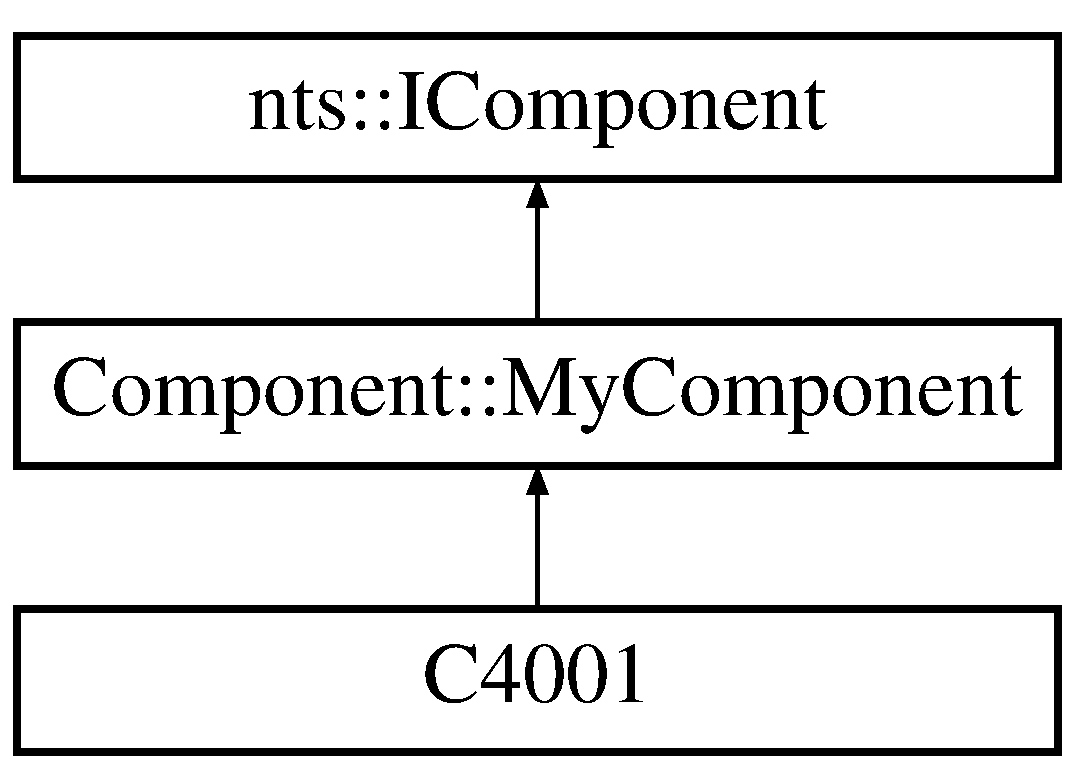
\includegraphics[height=3.000000cm]{classC4001}
\end{center}
\end{figure}
\subsection*{Public Member Functions}
\begin{DoxyCompactItemize}
\item 
\mbox{\hyperlink{classC4001_a3d1e79c23128b34f32bd941682ea2e66}{C4001}} ()
\begin{DoxyCompactList}\small\item\em Component 4001 Constructor. \end{DoxyCompactList}\item 
\mbox{\Hypertarget{classC4001_a22bee99372f97c18a9335ef398c9cc51}\label{classC4001_a22bee99372f97c18a9335ef398c9cc51}} 
\mbox{\hyperlink{classC4001_a22bee99372f97c18a9335ef398c9cc51}{$\sim$\+C4001}} ()
\begin{DoxyCompactList}\small\item\em Component 4001 Destructor. \end{DoxyCompactList}\item 
nts\+::\+Tristate \mbox{\hyperlink{classC4001_a2f3b7d19b418d8fbcfe08ed94b6a3e3a}{compute}} (std\+::size\+\_\+t pin=1) override
\begin{DoxyCompactList}\small\item\em Compute. \end{DoxyCompactList}\item 
void \mbox{\hyperlink{classC4001_acd977a0811ba00a202d346e551348f46}{set\+Link}} (std\+::size\+\_\+t pin, \mbox{\hyperlink{classnts_1_1IComponent}{nts\+::\+I\+Component}} \&other, std\+::size\+\_\+t other\+Pin) final
\begin{DoxyCompactList}\small\item\em Set link method. \end{DoxyCompactList}\item 
void \mbox{\hyperlink{classC4001_a2c2b7a726830f95515ce5538c1508b1f}{dump}} () const noexcept override
\begin{DoxyCompactList}\small\item\em Display information. \end{DoxyCompactList}\item 
void \mbox{\hyperlink{classC4001_a6cd7ce77dbd4bba7cbbdca0bc14cdb3b}{set\+Input}} (std\+::size\+\_\+t pin, \mbox{\hyperlink{classnts_1_1IComponent}{nts\+::\+I\+Component}} \&other, std\+::size\+\_\+t other\+Pin) final
\begin{DoxyCompactList}\small\item\em Set input link method. \end{DoxyCompactList}\item 
void \mbox{\hyperlink{classC4001_a6fc874b1c8f66481441214e6adc473fd}{set\+Output}} (std\+::size\+\_\+t pin, \mbox{\hyperlink{classnts_1_1IComponent}{nts\+::\+I\+Component}} \&other, std\+::size\+\_\+t other\+Pin) final
\begin{DoxyCompactList}\small\item\em Set output link method. \end{DoxyCompactList}\end{DoxyCompactItemize}
\subsection*{Additional Inherited Members}


\subsection{Detailed Description}
Quad 2-\/input N\+OR gate. 

\subsection{Constructor \& Destructor Documentation}
\mbox{\Hypertarget{classC4001_a3d1e79c23128b34f32bd941682ea2e66}\label{classC4001_a3d1e79c23128b34f32bd941682ea2e66}} 
\index{C4001@{C4001}!C4001@{C4001}}
\index{C4001@{C4001}!C4001@{C4001}}
\subsubsection{\texorpdfstring{C4001()}{C4001()}}
{\footnotesize\ttfamily C4001\+::\+C4001 (\begin{DoxyParamCaption}{ }\end{DoxyParamCaption})}



Component 4001 Constructor. 

Initializes four N\+OR gates with their own output and input pins. 

\subsection{Member Function Documentation}
\mbox{\Hypertarget{classC4001_a2f3b7d19b418d8fbcfe08ed94b6a3e3a}\label{classC4001_a2f3b7d19b418d8fbcfe08ed94b6a3e3a}} 
\index{C4001@{C4001}!compute@{compute}}
\index{compute@{compute}!C4001@{C4001}}
\subsubsection{\texorpdfstring{compute()}{compute()}}
{\footnotesize\ttfamily nts\+::\+Tristate C4001\+::compute (\begin{DoxyParamCaption}\item[{std\+::size\+\_\+t}]{pin = {\ttfamily 1} }\end{DoxyParamCaption})\hspace{0.3cm}{\ttfamily [override]}, {\ttfamily [virtual]}}



Compute. 

Searches for the door containing the requested pin and calculates the exit status.


\begin{DoxyParams}{Parameters}
{\em pin} & Pin requested \\
\hline
\end{DoxyParams}
\begin{DoxyReturn}{Returns}
\mbox{\hyperlink{classOutput}{Output}}\textquotesingle{}s door state. Can be true, false or undefined 
\end{DoxyReturn}


Implements \mbox{\hyperlink{classnts_1_1IComponent}{nts\+::\+I\+Component}}.

\mbox{\Hypertarget{classC4001_a2c2b7a726830f95515ce5538c1508b1f}\label{classC4001_a2c2b7a726830f95515ce5538c1508b1f}} 
\index{C4001@{C4001}!dump@{dump}}
\index{dump@{dump}!C4001@{C4001}}
\subsubsection{\texorpdfstring{dump()}{dump()}}
{\footnotesize\ttfamily void C4001\+::dump (\begin{DoxyParamCaption}{ }\end{DoxyParamCaption}) const\hspace{0.3cm}{\ttfamily [override]}, {\ttfamily [virtual]}, {\ttfamily [noexcept]}}



Display information. 

Display all pins state and link of component 4001 

Implements \mbox{\hyperlink{classnts_1_1IComponent}{nts\+::\+I\+Component}}.

\mbox{\Hypertarget{classC4001_a6cd7ce77dbd4bba7cbbdca0bc14cdb3b}\label{classC4001_a6cd7ce77dbd4bba7cbbdca0bc14cdb3b}} 
\index{C4001@{C4001}!set\+Input@{set\+Input}}
\index{set\+Input@{set\+Input}!C4001@{C4001}}
\subsubsection{\texorpdfstring{set\+Input()}{setInput()}}
{\footnotesize\ttfamily void C4001\+::set\+Input (\begin{DoxyParamCaption}\item[{std\+::size\+\_\+t}]{pin,  }\item[{\mbox{\hyperlink{classnts_1_1IComponent}{nts\+::\+I\+Component}} \&}]{other,  }\item[{std\+::size\+\_\+t}]{other\+Pin }\end{DoxyParamCaption})\hspace{0.3cm}{\ttfamily [final]}, {\ttfamily [virtual]}}



Set input link method. 

Method call by another component to bind to component 4001\textquotesingle{}s input


\begin{DoxyParams}{Parameters}
{\em pin} & Pin linked \\
\hline
{\em other} & Other Component \\
\hline
{\em other\+Pin} & Ohter component pin \\
\hline
\end{DoxyParams}


Implements \mbox{\hyperlink{classnts_1_1IComponent}{nts\+::\+I\+Component}}.

\mbox{\Hypertarget{classC4001_acd977a0811ba00a202d346e551348f46}\label{classC4001_acd977a0811ba00a202d346e551348f46}} 
\index{C4001@{C4001}!set\+Link@{set\+Link}}
\index{set\+Link@{set\+Link}!C4001@{C4001}}
\subsubsection{\texorpdfstring{set\+Link()}{setLink()}}
{\footnotesize\ttfamily void C4001\+::set\+Link (\begin{DoxyParamCaption}\item[{std\+::size\+\_\+t}]{pin,  }\item[{\mbox{\hyperlink{classnts_1_1IComponent}{nts\+::\+I\+Component}} \&}]{other,  }\item[{std\+::size\+\_\+t}]{other\+Pin }\end{DoxyParamCaption})\hspace{0.3cm}{\ttfamily [final]}, {\ttfamily [virtual]}}



Set link method. 

Link this component to another


\begin{DoxyParams}{Parameters}
{\em pin} & Component pin that needs to be linked \\
\hline
{\em other} & The other Component \\
\hline
{\em other\+Pin} & The other component pin \\
\hline
\end{DoxyParams}


Implements \mbox{\hyperlink{classnts_1_1IComponent}{nts\+::\+I\+Component}}.

\mbox{\Hypertarget{classC4001_a6fc874b1c8f66481441214e6adc473fd}\label{classC4001_a6fc874b1c8f66481441214e6adc473fd}} 
\index{C4001@{C4001}!set\+Output@{set\+Output}}
\index{set\+Output@{set\+Output}!C4001@{C4001}}
\subsubsection{\texorpdfstring{set\+Output()}{setOutput()}}
{\footnotesize\ttfamily void C4001\+::set\+Output (\begin{DoxyParamCaption}\item[{std\+::size\+\_\+t}]{pin,  }\item[{\mbox{\hyperlink{classnts_1_1IComponent}{nts\+::\+I\+Component}} \&}]{other,  }\item[{std\+::size\+\_\+t}]{other\+Pin }\end{DoxyParamCaption})\hspace{0.3cm}{\ttfamily [final]}, {\ttfamily [virtual]}}



Set output link method. 

Method call by another component to bind to component 4001\textquotesingle{}s output


\begin{DoxyParams}{Parameters}
{\em pin} & Pin linked \\
\hline
{\em other} & Other Component \\
\hline
{\em other\+Pin} & Ohter component pin \\
\hline
\end{DoxyParams}


Implements \mbox{\hyperlink{classnts_1_1IComponent}{nts\+::\+I\+Component}}.



The documentation for this class was generated from the following files\+:\begin{DoxyCompactItemize}
\item 
Include/\mbox{\hyperlink{C4001_8hpp}{C4001.\+hpp}}\item 
Src/\+Components/C4001.\+cpp\end{DoxyCompactItemize}

\hypertarget{classC4011}{}\section{C4011 Class Reference}
\label{classC4011}\index{C4011@{C4011}}


Quad 2-\/input N\+A\+ND gate.  




{\ttfamily \#include $<$C4011.\+hpp$>$}

Inheritance diagram for C4011\+:\begin{figure}[H]
\begin{center}
\leavevmode
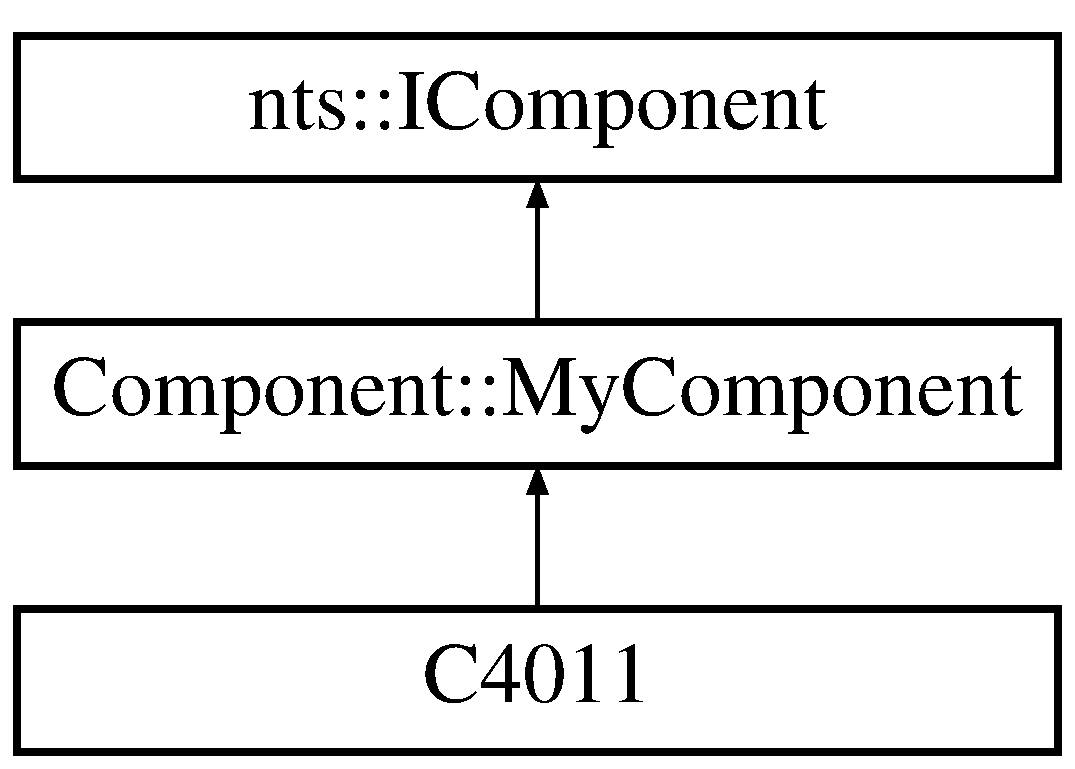
\includegraphics[height=3.000000cm]{classC4011}
\end{center}
\end{figure}
\subsection*{Public Member Functions}
\begin{DoxyCompactItemize}
\item 
\mbox{\hyperlink{classC4011_a179e783e10dea1e6caa775991ac90793}{C4011}} ()
\begin{DoxyCompactList}\small\item\em Component 4011 Constructor. \end{DoxyCompactList}\item 
\mbox{\Hypertarget{classC4011_adde3fe4950560251040f5b1710e22d2a}\label{classC4011_adde3fe4950560251040f5b1710e22d2a}} 
\mbox{\hyperlink{classC4011_adde3fe4950560251040f5b1710e22d2a}{$\sim$\+C4011}} ()
\begin{DoxyCompactList}\small\item\em Component 4011 Destructor. \end{DoxyCompactList}\item 
nts\+::\+Tristate \mbox{\hyperlink{classC4011_a1ed653298a52928ef7406c8f6817cbf3}{compute}} (std\+::size\+\_\+t pin=1) override
\begin{DoxyCompactList}\small\item\em Compute. \end{DoxyCompactList}\item 
void \mbox{\hyperlink{classC4011_a3fe0a0ef26a45324f11099c9b0ffa64c}{set\+Link}} (std\+::size\+\_\+t pin, \mbox{\hyperlink{classnts_1_1IComponent}{nts\+::\+I\+Component}} \&other, std\+::size\+\_\+t other\+Pin) final
\begin{DoxyCompactList}\small\item\em Set link method. \end{DoxyCompactList}\item 
void \mbox{\hyperlink{classC4011_a9aa9544c43493bcdf329aea1e475bfd5}{dump}} () const noexcept override
\begin{DoxyCompactList}\small\item\em Display information. \end{DoxyCompactList}\item 
void \mbox{\hyperlink{classC4011_a35c72f2ad0d4d0d90de38570901bfcf4}{set\+Input}} (std\+::size\+\_\+t pin, \mbox{\hyperlink{classnts_1_1IComponent}{nts\+::\+I\+Component}} \&other, std\+::size\+\_\+t other\+Pin) final
\begin{DoxyCompactList}\small\item\em Set input link method. \end{DoxyCompactList}\item 
void \mbox{\hyperlink{classC4011_a1d0a9e02002f0ad353c3d7357a6a625e}{set\+Output}} (std\+::size\+\_\+t pin, \mbox{\hyperlink{classnts_1_1IComponent}{nts\+::\+I\+Component}} \&other, std\+::size\+\_\+t other\+Pin) final
\begin{DoxyCompactList}\small\item\em Set output link method. \end{DoxyCompactList}\end{DoxyCompactItemize}
\subsection*{Additional Inherited Members}


\subsection{Detailed Description}
Quad 2-\/input N\+A\+ND gate. 

\subsection{Constructor \& Destructor Documentation}
\mbox{\Hypertarget{classC4011_a179e783e10dea1e6caa775991ac90793}\label{classC4011_a179e783e10dea1e6caa775991ac90793}} 
\index{C4011@{C4011}!C4011@{C4011}}
\index{C4011@{C4011}!C4011@{C4011}}
\subsubsection{\texorpdfstring{C4011()}{C4011()}}
{\footnotesize\ttfamily C4011\+::\+C4011 (\begin{DoxyParamCaption}{ }\end{DoxyParamCaption})}



Component 4011 Constructor. 

Initializes four N\+A\+ND gates with their own output and input pins. 

\subsection{Member Function Documentation}
\mbox{\Hypertarget{classC4011_a1ed653298a52928ef7406c8f6817cbf3}\label{classC4011_a1ed653298a52928ef7406c8f6817cbf3}} 
\index{C4011@{C4011}!compute@{compute}}
\index{compute@{compute}!C4011@{C4011}}
\subsubsection{\texorpdfstring{compute()}{compute()}}
{\footnotesize\ttfamily nts\+::\+Tristate C4011\+::compute (\begin{DoxyParamCaption}\item[{std\+::size\+\_\+t}]{pin = {\ttfamily 1} }\end{DoxyParamCaption})\hspace{0.3cm}{\ttfamily [override]}, {\ttfamily [virtual]}}



Compute. 

Searches for the door containing the requested pin and calculates the exit status.


\begin{DoxyParams}{Parameters}
{\em pin} & Pin requested \\
\hline
\end{DoxyParams}
\begin{DoxyReturn}{Returns}
\mbox{\hyperlink{classOutput}{Output}}\textquotesingle{}s door state. Can be true, false or undefined 
\end{DoxyReturn}


Implements \mbox{\hyperlink{classnts_1_1IComponent}{nts\+::\+I\+Component}}.

\mbox{\Hypertarget{classC4011_a9aa9544c43493bcdf329aea1e475bfd5}\label{classC4011_a9aa9544c43493bcdf329aea1e475bfd5}} 
\index{C4011@{C4011}!dump@{dump}}
\index{dump@{dump}!C4011@{C4011}}
\subsubsection{\texorpdfstring{dump()}{dump()}}
{\footnotesize\ttfamily void C4011\+::dump (\begin{DoxyParamCaption}{ }\end{DoxyParamCaption}) const\hspace{0.3cm}{\ttfamily [override]}, {\ttfamily [virtual]}, {\ttfamily [noexcept]}}



Display information. 

Display all pins state and link of component 4011 

Implements \mbox{\hyperlink{classnts_1_1IComponent}{nts\+::\+I\+Component}}.

\mbox{\Hypertarget{classC4011_a35c72f2ad0d4d0d90de38570901bfcf4}\label{classC4011_a35c72f2ad0d4d0d90de38570901bfcf4}} 
\index{C4011@{C4011}!set\+Input@{set\+Input}}
\index{set\+Input@{set\+Input}!C4011@{C4011}}
\subsubsection{\texorpdfstring{set\+Input()}{setInput()}}
{\footnotesize\ttfamily void C4011\+::set\+Input (\begin{DoxyParamCaption}\item[{std\+::size\+\_\+t}]{pin,  }\item[{\mbox{\hyperlink{classnts_1_1IComponent}{nts\+::\+I\+Component}} \&}]{other,  }\item[{std\+::size\+\_\+t}]{other\+Pin }\end{DoxyParamCaption})\hspace{0.3cm}{\ttfamily [final]}, {\ttfamily [virtual]}}



Set input link method. 

Method call by another component to bind to component 4001\textquotesingle{}s input


\begin{DoxyParams}{Parameters}
{\em pin} & Pin linked \\
\hline
{\em other} & Other Component \\
\hline
{\em other\+Pin} & Ohter component pin \\
\hline
\end{DoxyParams}


Implements \mbox{\hyperlink{classnts_1_1IComponent}{nts\+::\+I\+Component}}.

\mbox{\Hypertarget{classC4011_a3fe0a0ef26a45324f11099c9b0ffa64c}\label{classC4011_a3fe0a0ef26a45324f11099c9b0ffa64c}} 
\index{C4011@{C4011}!set\+Link@{set\+Link}}
\index{set\+Link@{set\+Link}!C4011@{C4011}}
\subsubsection{\texorpdfstring{set\+Link()}{setLink()}}
{\footnotesize\ttfamily void C4011\+::set\+Link (\begin{DoxyParamCaption}\item[{std\+::size\+\_\+t}]{pin,  }\item[{\mbox{\hyperlink{classnts_1_1IComponent}{nts\+::\+I\+Component}} \&}]{other,  }\item[{std\+::size\+\_\+t}]{other\+Pin }\end{DoxyParamCaption})\hspace{0.3cm}{\ttfamily [final]}, {\ttfamily [virtual]}}



Set link method. 

Link this component to another


\begin{DoxyParams}{Parameters}
{\em pin} & Component pin that needs to be linked \\
\hline
{\em other} & The other Component \\
\hline
{\em other\+Pin} & The other component pin \\
\hline
\end{DoxyParams}


Implements \mbox{\hyperlink{classnts_1_1IComponent}{nts\+::\+I\+Component}}.

\mbox{\Hypertarget{classC4011_a1d0a9e02002f0ad353c3d7357a6a625e}\label{classC4011_a1d0a9e02002f0ad353c3d7357a6a625e}} 
\index{C4011@{C4011}!set\+Output@{set\+Output}}
\index{set\+Output@{set\+Output}!C4011@{C4011}}
\subsubsection{\texorpdfstring{set\+Output()}{setOutput()}}
{\footnotesize\ttfamily void C4011\+::set\+Output (\begin{DoxyParamCaption}\item[{std\+::size\+\_\+t}]{pin,  }\item[{\mbox{\hyperlink{classnts_1_1IComponent}{nts\+::\+I\+Component}} \&}]{other,  }\item[{std\+::size\+\_\+t}]{other\+Pin }\end{DoxyParamCaption})\hspace{0.3cm}{\ttfamily [final]}, {\ttfamily [virtual]}}



Set output link method. 

Method call by another component to bind to component 4001\textquotesingle{}s output


\begin{DoxyParams}{Parameters}
{\em pin} & Pin linked \\
\hline
{\em other} & Other Component \\
\hline
{\em other\+Pin} & Ohter component pin \\
\hline
\end{DoxyParams}


Implements \mbox{\hyperlink{classnts_1_1IComponent}{nts\+::\+I\+Component}}.



The documentation for this class was generated from the following files\+:\begin{DoxyCompactItemize}
\item 
Include/\mbox{\hyperlink{C4011_8hpp}{C4011.\+hpp}}\item 
Src/\+Components/C4011.\+cpp\end{DoxyCompactItemize}

\hypertarget{classC4030}{}\section{C4030 Class Reference}
\label{classC4030}\index{C4030@{C4030}}


Quad 2-\/input E\+X\+C\+L\+U\+S\+I\+V\+E-\/\+OR gate.  




{\ttfamily \#include $<$C4030.\+hpp$>$}

Inheritance diagram for C4030\+:\begin{figure}[H]
\begin{center}
\leavevmode
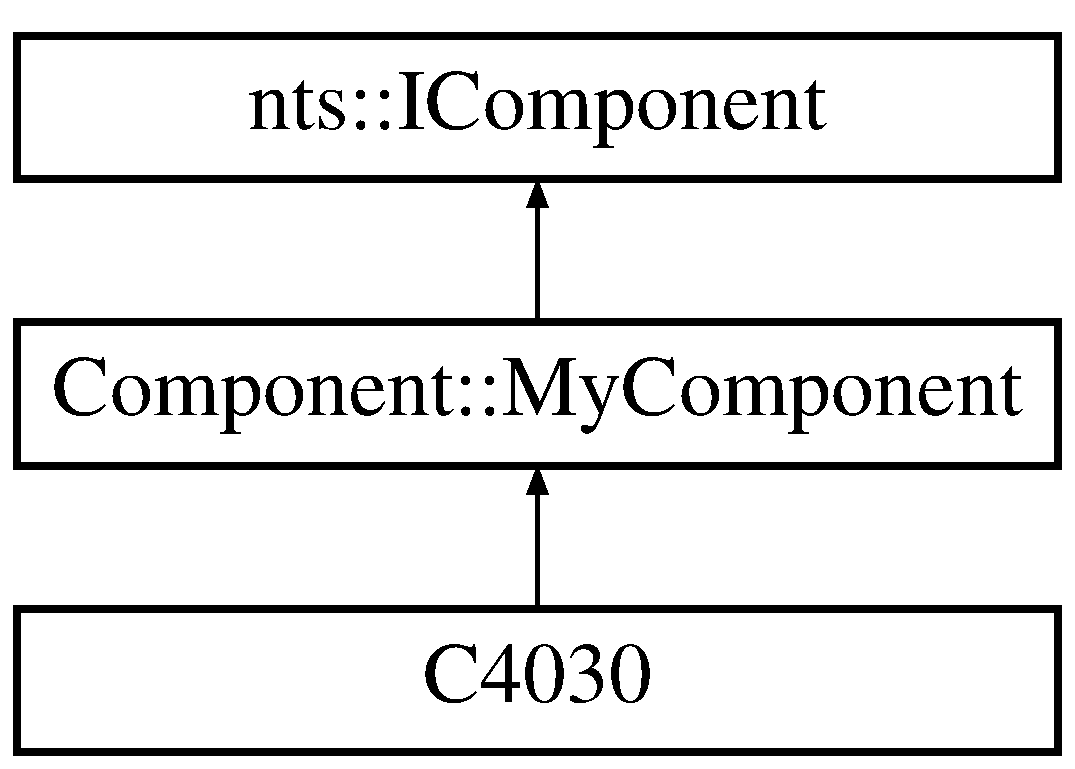
\includegraphics[height=3.000000cm]{classC4030}
\end{center}
\end{figure}
\subsection*{Public Member Functions}
\begin{DoxyCompactItemize}
\item 
\mbox{\hyperlink{classC4030_a4451260ff546d7daeefe6ea4ee2e877a}{C4030}} ()
\begin{DoxyCompactList}\small\item\em Component 4030 Constructor. \end{DoxyCompactList}\item 
\mbox{\Hypertarget{classC4030_a7c009fc75d3613b226f077dc96a1f26e}\label{classC4030_a7c009fc75d3613b226f077dc96a1f26e}} 
\mbox{\hyperlink{classC4030_a7c009fc75d3613b226f077dc96a1f26e}{$\sim$\+C4030}} ()
\begin{DoxyCompactList}\small\item\em Component 4030 Destructor. \end{DoxyCompactList}\item 
nts\+::\+Tristate \mbox{\hyperlink{classC4030_aa07ec80804c8109854c59da91c7ec636}{compute}} (std\+::size\+\_\+t pin=1) override
\begin{DoxyCompactList}\small\item\em Compute. \end{DoxyCompactList}\item 
void \mbox{\hyperlink{classC4030_ab6286489fdf747bc863223863e961a40}{set\+Link}} (std\+::size\+\_\+t pin, \mbox{\hyperlink{classnts_1_1IComponent}{nts\+::\+I\+Component}} \&other, std\+::size\+\_\+t other\+Pin) final
\begin{DoxyCompactList}\small\item\em Set link method. \end{DoxyCompactList}\item 
void \mbox{\hyperlink{classC4030_a55726374b18c0def739d5f25b19fe6c2}{dump}} () const noexcept override
\begin{DoxyCompactList}\small\item\em Display information. \end{DoxyCompactList}\item 
void \mbox{\hyperlink{classC4030_aa857c9828b1642c371976aaa01db4b74}{set\+Input}} (std\+::size\+\_\+t pin, \mbox{\hyperlink{classnts_1_1IComponent}{nts\+::\+I\+Component}} \&other, std\+::size\+\_\+t other\+Pin) final
\begin{DoxyCompactList}\small\item\em Set input link method. \end{DoxyCompactList}\item 
void \mbox{\hyperlink{classC4030_a233e02d922356fc378b6c9c807ce2e02}{set\+Output}} (std\+::size\+\_\+t pin, \mbox{\hyperlink{classnts_1_1IComponent}{nts\+::\+I\+Component}} \&other, std\+::size\+\_\+t other\+Pin) final
\begin{DoxyCompactList}\small\item\em Set output link method. \end{DoxyCompactList}\end{DoxyCompactItemize}
\subsection*{Additional Inherited Members}


\subsection{Detailed Description}
Quad 2-\/input E\+X\+C\+L\+U\+S\+I\+V\+E-\/\+OR gate. 

\subsection{Constructor \& Destructor Documentation}
\mbox{\Hypertarget{classC4030_a4451260ff546d7daeefe6ea4ee2e877a}\label{classC4030_a4451260ff546d7daeefe6ea4ee2e877a}} 
\index{C4030@{C4030}!C4030@{C4030}}
\index{C4030@{C4030}!C4030@{C4030}}
\subsubsection{\texorpdfstring{C4030()}{C4030()}}
{\footnotesize\ttfamily C4030\+::\+C4030 (\begin{DoxyParamCaption}{ }\end{DoxyParamCaption})}



Component 4030 Constructor. 

Initializes four E\+X\+C\+L\+U\+S\+I\+V\+E-\/\+OR gates with their own output and input pins. 

\subsection{Member Function Documentation}
\mbox{\Hypertarget{classC4030_aa07ec80804c8109854c59da91c7ec636}\label{classC4030_aa07ec80804c8109854c59da91c7ec636}} 
\index{C4030@{C4030}!compute@{compute}}
\index{compute@{compute}!C4030@{C4030}}
\subsubsection{\texorpdfstring{compute()}{compute()}}
{\footnotesize\ttfamily nts\+::\+Tristate C4030\+::compute (\begin{DoxyParamCaption}\item[{std\+::size\+\_\+t}]{pin = {\ttfamily 1} }\end{DoxyParamCaption})\hspace{0.3cm}{\ttfamily [override]}, {\ttfamily [virtual]}}



Compute. 

Searches for the door containing the requested pin and calculates the exit status.


\begin{DoxyParams}{Parameters}
{\em pin} & Pin requested \\
\hline
\end{DoxyParams}
\begin{DoxyReturn}{Returns}
\mbox{\hyperlink{classOutput}{Output}}\textquotesingle{}s door state. Can be true, false or undefined 
\end{DoxyReturn}


Implements \mbox{\hyperlink{classnts_1_1IComponent}{nts\+::\+I\+Component}}.

\mbox{\Hypertarget{classC4030_a55726374b18c0def739d5f25b19fe6c2}\label{classC4030_a55726374b18c0def739d5f25b19fe6c2}} 
\index{C4030@{C4030}!dump@{dump}}
\index{dump@{dump}!C4030@{C4030}}
\subsubsection{\texorpdfstring{dump()}{dump()}}
{\footnotesize\ttfamily void C4030\+::dump (\begin{DoxyParamCaption}{ }\end{DoxyParamCaption}) const\hspace{0.3cm}{\ttfamily [override]}, {\ttfamily [virtual]}, {\ttfamily [noexcept]}}



Display information. 

Display all pins state and link of component 4030 

Implements \mbox{\hyperlink{classnts_1_1IComponent}{nts\+::\+I\+Component}}.

\mbox{\Hypertarget{classC4030_aa857c9828b1642c371976aaa01db4b74}\label{classC4030_aa857c9828b1642c371976aaa01db4b74}} 
\index{C4030@{C4030}!set\+Input@{set\+Input}}
\index{set\+Input@{set\+Input}!C4030@{C4030}}
\subsubsection{\texorpdfstring{set\+Input()}{setInput()}}
{\footnotesize\ttfamily void C4030\+::set\+Input (\begin{DoxyParamCaption}\item[{std\+::size\+\_\+t}]{pin,  }\item[{\mbox{\hyperlink{classnts_1_1IComponent}{nts\+::\+I\+Component}} \&}]{other,  }\item[{std\+::size\+\_\+t}]{other\+Pin }\end{DoxyParamCaption})\hspace{0.3cm}{\ttfamily [final]}, {\ttfamily [virtual]}}



Set input link method. 

Method call by another component to bind to component 4030\textquotesingle{}s input


\begin{DoxyParams}{Parameters}
{\em pin} & Pin linked \\
\hline
{\em other} & Other Component \\
\hline
{\em other\+Pin} & Ohter component pin \\
\hline
\end{DoxyParams}


Implements \mbox{\hyperlink{classnts_1_1IComponent}{nts\+::\+I\+Component}}.

\mbox{\Hypertarget{classC4030_ab6286489fdf747bc863223863e961a40}\label{classC4030_ab6286489fdf747bc863223863e961a40}} 
\index{C4030@{C4030}!set\+Link@{set\+Link}}
\index{set\+Link@{set\+Link}!C4030@{C4030}}
\subsubsection{\texorpdfstring{set\+Link()}{setLink()}}
{\footnotesize\ttfamily void C4030\+::set\+Link (\begin{DoxyParamCaption}\item[{std\+::size\+\_\+t}]{pin,  }\item[{\mbox{\hyperlink{classnts_1_1IComponent}{nts\+::\+I\+Component}} \&}]{other,  }\item[{std\+::size\+\_\+t}]{other\+Pin }\end{DoxyParamCaption})\hspace{0.3cm}{\ttfamily [final]}, {\ttfamily [virtual]}}



Set link method. 

Link this component to another


\begin{DoxyParams}{Parameters}
{\em pin} & Component pin that needs to be linked \\
\hline
{\em other} & The other Component \\
\hline
{\em other\+Pin} & The other component pin \\
\hline
\end{DoxyParams}


Implements \mbox{\hyperlink{classnts_1_1IComponent}{nts\+::\+I\+Component}}.

\mbox{\Hypertarget{classC4030_a233e02d922356fc378b6c9c807ce2e02}\label{classC4030_a233e02d922356fc378b6c9c807ce2e02}} 
\index{C4030@{C4030}!set\+Output@{set\+Output}}
\index{set\+Output@{set\+Output}!C4030@{C4030}}
\subsubsection{\texorpdfstring{set\+Output()}{setOutput()}}
{\footnotesize\ttfamily void C4030\+::set\+Output (\begin{DoxyParamCaption}\item[{std\+::size\+\_\+t}]{pin,  }\item[{\mbox{\hyperlink{classnts_1_1IComponent}{nts\+::\+I\+Component}} \&}]{other,  }\item[{std\+::size\+\_\+t}]{other\+Pin }\end{DoxyParamCaption})\hspace{0.3cm}{\ttfamily [final]}, {\ttfamily [virtual]}}



Set output link method. 

Method call by another component to bind to component 4030\textquotesingle{}s output


\begin{DoxyParams}{Parameters}
{\em pin} & Pin linked \\
\hline
{\em other} & Other Component \\
\hline
{\em other\+Pin} & Ohter component pin \\
\hline
\end{DoxyParams}


Implements \mbox{\hyperlink{classnts_1_1IComponent}{nts\+::\+I\+Component}}.



The documentation for this class was generated from the following files\+:\begin{DoxyCompactItemize}
\item 
Include/\mbox{\hyperlink{C4030_8hpp}{C4030.\+hpp}}\item 
Src/\+Components/C4030.\+cpp\end{DoxyCompactItemize}

\hypertarget{classC4071}{}\section{C4071 Class Reference}
\label{classC4071}\index{C4071@{C4071}}


Quad 2-\/input OR gate.  




{\ttfamily \#include $<$C4071.\+hpp$>$}

Inheritance diagram for C4071\+:\begin{figure}[H]
\begin{center}
\leavevmode
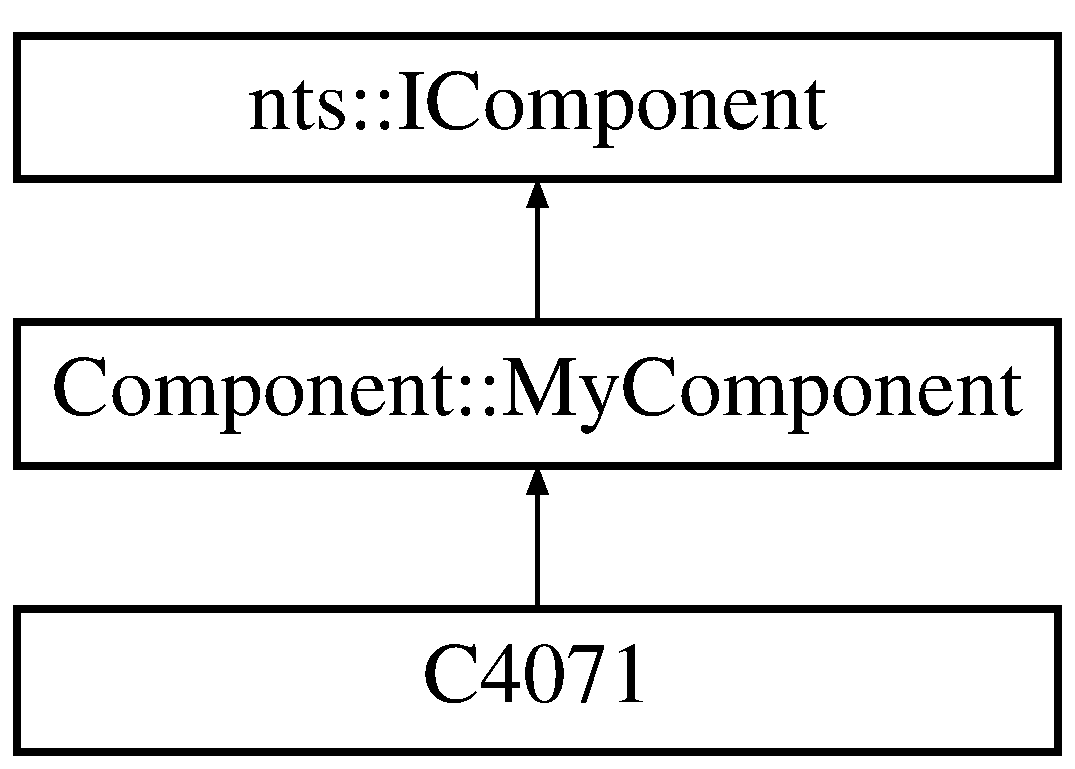
\includegraphics[height=3.000000cm]{classC4071}
\end{center}
\end{figure}
\subsection*{Public Member Functions}
\begin{DoxyCompactItemize}
\item 
\mbox{\hyperlink{classC4071_ac33d5f23fd2f325b4e67c1107971e8d5}{C4071}} ()
\begin{DoxyCompactList}\small\item\em Component 4071 Constructor. \end{DoxyCompactList}\item 
\mbox{\Hypertarget{classC4071_a5e437df39bafa4b93da5d66c1dcb9cb3}\label{classC4071_a5e437df39bafa4b93da5d66c1dcb9cb3}} 
\mbox{\hyperlink{classC4071_a5e437df39bafa4b93da5d66c1dcb9cb3}{$\sim$\+C4071}} ()
\begin{DoxyCompactList}\small\item\em Component 4071 Destructor. \end{DoxyCompactList}\item 
nts\+::\+Tristate \mbox{\hyperlink{classC4071_af027f99834e11ebf7eed3140b25011b7}{compute}} (std\+::size\+\_\+t pin=1) override
\begin{DoxyCompactList}\small\item\em Compute. \end{DoxyCompactList}\item 
void \mbox{\hyperlink{classC4071_af9bec6200cffbba1c5a9a1c904869c20}{set\+Link}} (std\+::size\+\_\+t pin, \mbox{\hyperlink{classnts_1_1IComponent}{nts\+::\+I\+Component}} \&other, std\+::size\+\_\+t other\+Pin) final
\begin{DoxyCompactList}\small\item\em Set link method. \end{DoxyCompactList}\item 
void \mbox{\hyperlink{classC4071_a495ed3223c0e31b92abb9f8c9785c789}{dump}} () const noexcept override
\begin{DoxyCompactList}\small\item\em Display information. \end{DoxyCompactList}\item 
void \mbox{\hyperlink{classC4071_a48d9c405a1d4ef621b971cdbfd48d65f}{set\+Input}} (std\+::size\+\_\+t pin, \mbox{\hyperlink{classnts_1_1IComponent}{nts\+::\+I\+Component}} \&other, std\+::size\+\_\+t other\+Pin) final
\begin{DoxyCompactList}\small\item\em Set input link method. \end{DoxyCompactList}\item 
void \mbox{\hyperlink{classC4071_abbedfad8c619e64d3f63c0a9731d82e6}{set\+Output}} (std\+::size\+\_\+t pin, \mbox{\hyperlink{classnts_1_1IComponent}{nts\+::\+I\+Component}} \&other, std\+::size\+\_\+t other\+Pin) final
\begin{DoxyCompactList}\small\item\em Set output link method. \end{DoxyCompactList}\end{DoxyCompactItemize}
\subsection*{Additional Inherited Members}


\subsection{Detailed Description}
Quad 2-\/input OR gate. 

\subsection{Constructor \& Destructor Documentation}
\mbox{\Hypertarget{classC4071_ac33d5f23fd2f325b4e67c1107971e8d5}\label{classC4071_ac33d5f23fd2f325b4e67c1107971e8d5}} 
\index{C4071@{C4071}!C4071@{C4071}}
\index{C4071@{C4071}!C4071@{C4071}}
\subsubsection{\texorpdfstring{C4071()}{C4071()}}
{\footnotesize\ttfamily C4071\+::\+C4071 (\begin{DoxyParamCaption}{ }\end{DoxyParamCaption})}



Component 4071 Constructor. 

Initializes four OR gates with their own output and input pins. 

\subsection{Member Function Documentation}
\mbox{\Hypertarget{classC4071_af027f99834e11ebf7eed3140b25011b7}\label{classC4071_af027f99834e11ebf7eed3140b25011b7}} 
\index{C4071@{C4071}!compute@{compute}}
\index{compute@{compute}!C4071@{C4071}}
\subsubsection{\texorpdfstring{compute()}{compute()}}
{\footnotesize\ttfamily nts\+::\+Tristate C4071\+::compute (\begin{DoxyParamCaption}\item[{std\+::size\+\_\+t}]{pin = {\ttfamily 1} }\end{DoxyParamCaption})\hspace{0.3cm}{\ttfamily [override]}, {\ttfamily [virtual]}}



Compute. 

Searches for the door containing the requested pin and calculates the exit status.


\begin{DoxyParams}{Parameters}
{\em pin} & Pin requested \\
\hline
\end{DoxyParams}
\begin{DoxyReturn}{Returns}
\mbox{\hyperlink{classOutput}{Output}}\textquotesingle{}s door state. Can be true, false or undefined 
\end{DoxyReturn}


Implements \mbox{\hyperlink{classnts_1_1IComponent}{nts\+::\+I\+Component}}.

\mbox{\Hypertarget{classC4071_a495ed3223c0e31b92abb9f8c9785c789}\label{classC4071_a495ed3223c0e31b92abb9f8c9785c789}} 
\index{C4071@{C4071}!dump@{dump}}
\index{dump@{dump}!C4071@{C4071}}
\subsubsection{\texorpdfstring{dump()}{dump()}}
{\footnotesize\ttfamily void C4071\+::dump (\begin{DoxyParamCaption}{ }\end{DoxyParamCaption}) const\hspace{0.3cm}{\ttfamily [override]}, {\ttfamily [virtual]}, {\ttfamily [noexcept]}}



Display information. 

Display all pins state and link of component 4071 

Implements \mbox{\hyperlink{classnts_1_1IComponent}{nts\+::\+I\+Component}}.

\mbox{\Hypertarget{classC4071_a48d9c405a1d4ef621b971cdbfd48d65f}\label{classC4071_a48d9c405a1d4ef621b971cdbfd48d65f}} 
\index{C4071@{C4071}!set\+Input@{set\+Input}}
\index{set\+Input@{set\+Input}!C4071@{C4071}}
\subsubsection{\texorpdfstring{set\+Input()}{setInput()}}
{\footnotesize\ttfamily void C4071\+::set\+Input (\begin{DoxyParamCaption}\item[{std\+::size\+\_\+t}]{pin,  }\item[{\mbox{\hyperlink{classnts_1_1IComponent}{nts\+::\+I\+Component}} \&}]{other,  }\item[{std\+::size\+\_\+t}]{other\+Pin }\end{DoxyParamCaption})\hspace{0.3cm}{\ttfamily [final]}, {\ttfamily [virtual]}}



Set input link method. 

Method call by another component to bind to component 4071\textquotesingle{}s input


\begin{DoxyParams}{Parameters}
{\em pin} & Pin linked \\
\hline
{\em other} & Other Component \\
\hline
{\em other\+Pin} & Ohter component pin \\
\hline
\end{DoxyParams}


Implements \mbox{\hyperlink{classnts_1_1IComponent}{nts\+::\+I\+Component}}.

\mbox{\Hypertarget{classC4071_af9bec6200cffbba1c5a9a1c904869c20}\label{classC4071_af9bec6200cffbba1c5a9a1c904869c20}} 
\index{C4071@{C4071}!set\+Link@{set\+Link}}
\index{set\+Link@{set\+Link}!C4071@{C4071}}
\subsubsection{\texorpdfstring{set\+Link()}{setLink()}}
{\footnotesize\ttfamily void C4071\+::set\+Link (\begin{DoxyParamCaption}\item[{std\+::size\+\_\+t}]{pin,  }\item[{\mbox{\hyperlink{classnts_1_1IComponent}{nts\+::\+I\+Component}} \&}]{other,  }\item[{std\+::size\+\_\+t}]{other\+Pin }\end{DoxyParamCaption})\hspace{0.3cm}{\ttfamily [final]}, {\ttfamily [virtual]}}



Set link method. 

Link this component to another


\begin{DoxyParams}{Parameters}
{\em pin} & Component pin that needs to be linked \\
\hline
{\em other} & The other Component \\
\hline
{\em other\+Pin} & The other component pin \\
\hline
\end{DoxyParams}


Implements \mbox{\hyperlink{classnts_1_1IComponent}{nts\+::\+I\+Component}}.

\mbox{\Hypertarget{classC4071_abbedfad8c619e64d3f63c0a9731d82e6}\label{classC4071_abbedfad8c619e64d3f63c0a9731d82e6}} 
\index{C4071@{C4071}!set\+Output@{set\+Output}}
\index{set\+Output@{set\+Output}!C4071@{C4071}}
\subsubsection{\texorpdfstring{set\+Output()}{setOutput()}}
{\footnotesize\ttfamily void C4071\+::set\+Output (\begin{DoxyParamCaption}\item[{std\+::size\+\_\+t}]{pin,  }\item[{\mbox{\hyperlink{classnts_1_1IComponent}{nts\+::\+I\+Component}} \&}]{other,  }\item[{std\+::size\+\_\+t}]{other\+Pin }\end{DoxyParamCaption})\hspace{0.3cm}{\ttfamily [final]}, {\ttfamily [virtual]}}



Set output link method. 

Method call by another component to bind to component 4071\textquotesingle{}s output


\begin{DoxyParams}{Parameters}
{\em pin} & Pin linked \\
\hline
{\em other} & Other Component \\
\hline
{\em other\+Pin} & Ohter component pin \\
\hline
\end{DoxyParams}


Implements \mbox{\hyperlink{classnts_1_1IComponent}{nts\+::\+I\+Component}}.



The documentation for this class was generated from the following files\+:\begin{DoxyCompactItemize}
\item 
Include/\mbox{\hyperlink{C4071_8hpp}{C4071.\+hpp}}\item 
Src/\+Components/C4071.\+cpp\end{DoxyCompactItemize}

\hypertarget{classC4081}{}\section{C4081 Class Reference}
\label{classC4081}\index{C4081@{C4081}}


Quad 2-\/input A\+ND gate.  




{\ttfamily \#include $<$C4081.\+hpp$>$}

Inheritance diagram for C4081\+:\begin{figure}[H]
\begin{center}
\leavevmode
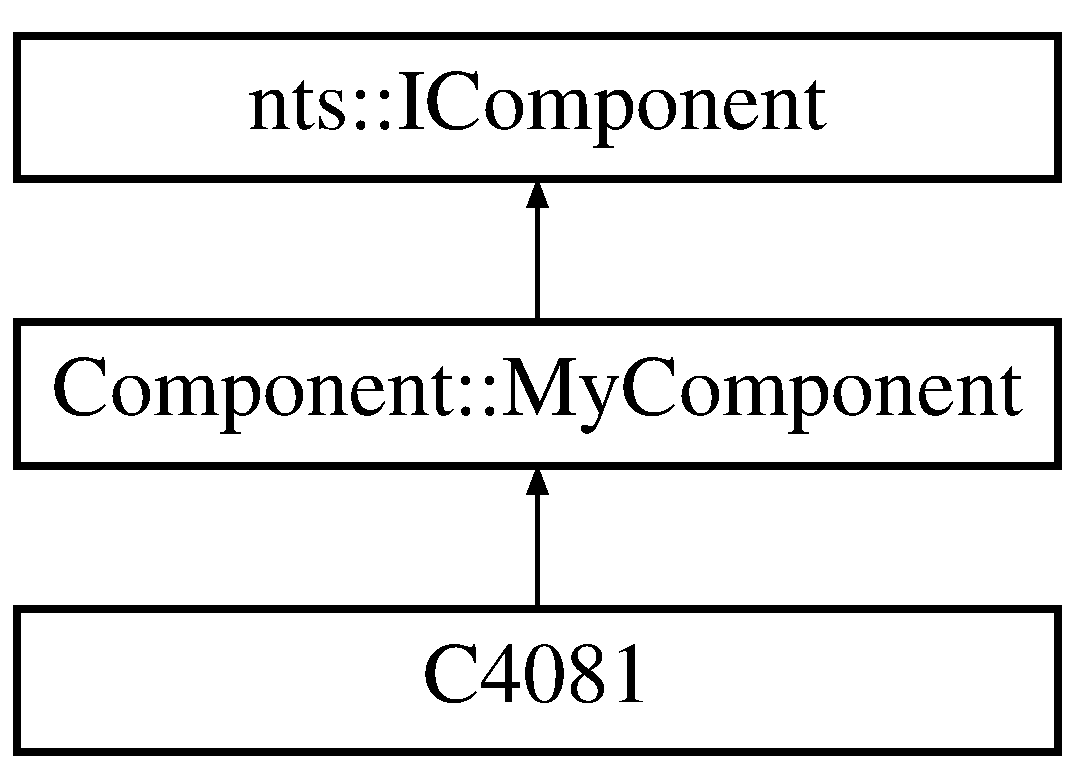
\includegraphics[height=3.000000cm]{classC4081}
\end{center}
\end{figure}
\subsection*{Public Member Functions}
\begin{DoxyCompactItemize}
\item 
\mbox{\hyperlink{classC4081_afa84f979826cb257f236fee5a92b4af6}{C4081}} ()
\begin{DoxyCompactList}\small\item\em Component 4081 Constructor. \end{DoxyCompactList}\item 
\mbox{\Hypertarget{classC4081_a960a6a35c939ebd584d54a7b54daa0a7}\label{classC4081_a960a6a35c939ebd584d54a7b54daa0a7}} 
\mbox{\hyperlink{classC4081_a960a6a35c939ebd584d54a7b54daa0a7}{$\sim$\+C4081}} ()
\begin{DoxyCompactList}\small\item\em Component 4081 Destructor. \end{DoxyCompactList}\item 
nts\+::\+Tristate \mbox{\hyperlink{classC4081_a1c32e380468dd0ccfe9da7fa6432d31a}{compute}} (std\+::size\+\_\+t pin=1) override
\begin{DoxyCompactList}\small\item\em Compute. \end{DoxyCompactList}\item 
void \mbox{\hyperlink{classC4081_a21e38e780f876bcbee9e522e621654a3}{set\+Link}} (std\+::size\+\_\+t pin, \mbox{\hyperlink{classnts_1_1IComponent}{nts\+::\+I\+Component}} \&other, std\+::size\+\_\+t other\+Pin) final
\begin{DoxyCompactList}\small\item\em Set link method. \end{DoxyCompactList}\item 
void \mbox{\hyperlink{classC4081_a0ef9e2164c25c6aed2f2e3a54d7417fa}{dump}} () const noexcept override
\begin{DoxyCompactList}\small\item\em Display information. \end{DoxyCompactList}\item 
void \mbox{\hyperlink{classC4081_a21323fd9bab910718335dc009b2b90c2}{set\+Input}} (std\+::size\+\_\+t pin, \mbox{\hyperlink{classnts_1_1IComponent}{nts\+::\+I\+Component}} \&other, std\+::size\+\_\+t other\+Pin) final
\begin{DoxyCompactList}\small\item\em Set input link method. \end{DoxyCompactList}\item 
void \mbox{\hyperlink{classC4081_af17058a91dbb223bf38c745cd7287557}{set\+Output}} (std\+::size\+\_\+t pin, \mbox{\hyperlink{classnts_1_1IComponent}{nts\+::\+I\+Component}} \&other, std\+::size\+\_\+t other\+Pin) final
\begin{DoxyCompactList}\small\item\em Set output link method. \end{DoxyCompactList}\end{DoxyCompactItemize}
\subsection*{Additional Inherited Members}


\subsection{Detailed Description}
Quad 2-\/input A\+ND gate. 

\subsection{Constructor \& Destructor Documentation}
\mbox{\Hypertarget{classC4081_afa84f979826cb257f236fee5a92b4af6}\label{classC4081_afa84f979826cb257f236fee5a92b4af6}} 
\index{C4081@{C4081}!C4081@{C4081}}
\index{C4081@{C4081}!C4081@{C4081}}
\subsubsection{\texorpdfstring{C4081()}{C4081()}}
{\footnotesize\ttfamily C4081\+::\+C4081 (\begin{DoxyParamCaption}{ }\end{DoxyParamCaption})}



Component 4081 Constructor. 

Initializes four A\+ND gates with their own output and input pins. 

\subsection{Member Function Documentation}
\mbox{\Hypertarget{classC4081_a1c32e380468dd0ccfe9da7fa6432d31a}\label{classC4081_a1c32e380468dd0ccfe9da7fa6432d31a}} 
\index{C4081@{C4081}!compute@{compute}}
\index{compute@{compute}!C4081@{C4081}}
\subsubsection{\texorpdfstring{compute()}{compute()}}
{\footnotesize\ttfamily nts\+::\+Tristate C4081\+::compute (\begin{DoxyParamCaption}\item[{std\+::size\+\_\+t}]{pin = {\ttfamily 1} }\end{DoxyParamCaption})\hspace{0.3cm}{\ttfamily [override]}, {\ttfamily [virtual]}}



Compute. 

Searches for the door containing the requested pin and calculates the exit status.


\begin{DoxyParams}{Parameters}
{\em pin} & Pin requested \\
\hline
\end{DoxyParams}
\begin{DoxyReturn}{Returns}
\mbox{\hyperlink{classOutput}{Output}}\textquotesingle{}s door state. Can be true, false or undefined 
\end{DoxyReturn}


Implements \mbox{\hyperlink{classnts_1_1IComponent}{nts\+::\+I\+Component}}.

\mbox{\Hypertarget{classC4081_a0ef9e2164c25c6aed2f2e3a54d7417fa}\label{classC4081_a0ef9e2164c25c6aed2f2e3a54d7417fa}} 
\index{C4081@{C4081}!dump@{dump}}
\index{dump@{dump}!C4081@{C4081}}
\subsubsection{\texorpdfstring{dump()}{dump()}}
{\footnotesize\ttfamily void C4081\+::dump (\begin{DoxyParamCaption}{ }\end{DoxyParamCaption}) const\hspace{0.3cm}{\ttfamily [override]}, {\ttfamily [virtual]}, {\ttfamily [noexcept]}}



Display information. 

Display all pins state and link of component 4081 

Implements \mbox{\hyperlink{classnts_1_1IComponent}{nts\+::\+I\+Component}}.

\mbox{\Hypertarget{classC4081_a21323fd9bab910718335dc009b2b90c2}\label{classC4081_a21323fd9bab910718335dc009b2b90c2}} 
\index{C4081@{C4081}!set\+Input@{set\+Input}}
\index{set\+Input@{set\+Input}!C4081@{C4081}}
\subsubsection{\texorpdfstring{set\+Input()}{setInput()}}
{\footnotesize\ttfamily void C4081\+::set\+Input (\begin{DoxyParamCaption}\item[{std\+::size\+\_\+t}]{pin,  }\item[{\mbox{\hyperlink{classnts_1_1IComponent}{nts\+::\+I\+Component}} \&}]{other,  }\item[{std\+::size\+\_\+t}]{other\+Pin }\end{DoxyParamCaption})\hspace{0.3cm}{\ttfamily [final]}, {\ttfamily [virtual]}}



Set input link method. 

Method call by another component to bind to component 4081\textquotesingle{}s input


\begin{DoxyParams}{Parameters}
{\em pin} & Pin linked \\
\hline
{\em other} & Other Component \\
\hline
{\em other\+Pin} & Ohter component pin \\
\hline
\end{DoxyParams}


Implements \mbox{\hyperlink{classnts_1_1IComponent}{nts\+::\+I\+Component}}.

\mbox{\Hypertarget{classC4081_a21e38e780f876bcbee9e522e621654a3}\label{classC4081_a21e38e780f876bcbee9e522e621654a3}} 
\index{C4081@{C4081}!set\+Link@{set\+Link}}
\index{set\+Link@{set\+Link}!C4081@{C4081}}
\subsubsection{\texorpdfstring{set\+Link()}{setLink()}}
{\footnotesize\ttfamily void C4081\+::set\+Link (\begin{DoxyParamCaption}\item[{std\+::size\+\_\+t}]{pin,  }\item[{\mbox{\hyperlink{classnts_1_1IComponent}{nts\+::\+I\+Component}} \&}]{other,  }\item[{std\+::size\+\_\+t}]{other\+Pin }\end{DoxyParamCaption})\hspace{0.3cm}{\ttfamily [final]}, {\ttfamily [virtual]}}



Set link method. 

Link this component to another


\begin{DoxyParams}{Parameters}
{\em pin} & Component pin that needs to be linked \\
\hline
{\em other} & The other Component \\
\hline
{\em other\+Pin} & The other component pin \\
\hline
\end{DoxyParams}


Implements \mbox{\hyperlink{classnts_1_1IComponent}{nts\+::\+I\+Component}}.

\mbox{\Hypertarget{classC4081_af17058a91dbb223bf38c745cd7287557}\label{classC4081_af17058a91dbb223bf38c745cd7287557}} 
\index{C4081@{C4081}!set\+Output@{set\+Output}}
\index{set\+Output@{set\+Output}!C4081@{C4081}}
\subsubsection{\texorpdfstring{set\+Output()}{setOutput()}}
{\footnotesize\ttfamily void C4081\+::set\+Output (\begin{DoxyParamCaption}\item[{std\+::size\+\_\+t}]{pin,  }\item[{\mbox{\hyperlink{classnts_1_1IComponent}{nts\+::\+I\+Component}} \&}]{other,  }\item[{std\+::size\+\_\+t}]{other\+Pin }\end{DoxyParamCaption})\hspace{0.3cm}{\ttfamily [final]}, {\ttfamily [virtual]}}



Set output link method. 

Method call by another component to bind to component 4081\textquotesingle{}s output


\begin{DoxyParams}{Parameters}
{\em pin} & Pin linked \\
\hline
{\em other} & Other Component \\
\hline
{\em other\+Pin} & Ohter component pin \\
\hline
\end{DoxyParams}


Implements \mbox{\hyperlink{classnts_1_1IComponent}{nts\+::\+I\+Component}}.



The documentation for this class was generated from the following files\+:\begin{DoxyCompactItemize}
\item 
Include/\mbox{\hyperlink{C4081_8hpp}{C4081.\+hpp}}\item 
Src/\+Components/C4081.\+cpp\end{DoxyCompactItemize}

\hypertarget{classParser_1_1Checker}{}\section{Parser\+:\+:Checker Class Reference}
\label{classParser_1_1Checker}\index{Parser\+::\+Checker@{Parser\+::\+Checker}}
\subsection*{Public Member Functions}
\begin{DoxyCompactItemize}
\item 
\mbox{\Hypertarget{classParser_1_1Checker_a57cef62f94c2f4bf0795e4d434dc6069}\label{classParser_1_1Checker_a57cef62f94c2f4bf0795e4d434dc6069}} 
{\bfseries Checker} (const container\+\_\+setting\+\_\+t \&chipset\+Info, const container\+\_\+link\+\_\+t \&all\+Links)
\item 
\mbox{\Hypertarget{classParser_1_1Checker_ae925eba41fa833edde25e1ef3dcd04c0}\label{classParser_1_1Checker_ae925eba41fa833edde25e1ef3dcd04c0}} 
{\bfseries Checker} (const container\+\_\+setting\+\_\+t \&chipset\+Info)
\item 
\mbox{\Hypertarget{classParser_1_1Checker_a87e0ce608ac90feaca458d66d224b1d2}\label{classParser_1_1Checker_a87e0ce608ac90feaca458d66d224b1d2}} 
{\bfseries Checker} (const container\+\_\+link\+\_\+t \&all\+Links)
\item 
\mbox{\Hypertarget{classParser_1_1Checker_a0aaff69ec0fdaffc339d34062707f839}\label{classParser_1_1Checker_a0aaff69ec0fdaffc339d34062707f839}} 
{\bfseries Checker} (const std\+::string \&line)
\item 
\mbox{\Hypertarget{classParser_1_1Checker_ad396a3c43a4c4c111052272b71710f35}\label{classParser_1_1Checker_ad396a3c43a4c4c111052272b71710f35}} 
void {\bfseries Check} ()
\item 
\mbox{\Hypertarget{classParser_1_1Checker_a342e5fae6d2a36377e3288258e3743a5}\label{classParser_1_1Checker_a342e5fae6d2a36377e3288258e3743a5}} 
void {\bfseries Check\+Names} () const
\item 
\mbox{\Hypertarget{classParser_1_1Checker_af19c4303b859db1347e24e3dc0f8177a}\label{classParser_1_1Checker_af19c4303b859db1347e24e3dc0f8177a}} 
void {\bfseries Check\+Type} () const
\item 
\mbox{\Hypertarget{classParser_1_1Checker_a7a9fbde5ddef9a6a679eb26d6cbeee6a}\label{classParser_1_1Checker_a7a9fbde5ddef9a6a679eb26d6cbeee6a}} 
void {\bfseries Check\+Outputs} () const
\item 
\mbox{\Hypertarget{classParser_1_1Checker_a63948e7c29a6d49a45132a79659d52ac}\label{classParser_1_1Checker_a63948e7c29a6d49a45132a79659d52ac}} 
void {\bfseries Check\+Links\+Multiple} () const
\item 
\mbox{\Hypertarget{classParser_1_1Checker_aa454723cd447e58073d2a44838aa87df}\label{classParser_1_1Checker_aa454723cd447e58073d2a44838aa87df}} 
bool {\bfseries Is\+Useless} () const
\end{DoxyCompactItemize}


The documentation for this class was generated from the following files\+:\begin{DoxyCompactItemize}
\item 
Include/Parser.\+hpp\item 
Src/\+Parser/Checker.\+cpp\end{DoxyCompactItemize}

\hypertarget{classCircuit}{}\section{Circuit Class Reference}
\label{classCircuit}\index{Circuit@{Circuit}}
Inheritance diagram for Circuit\+:\begin{figure}[H]
\begin{center}
\leavevmode
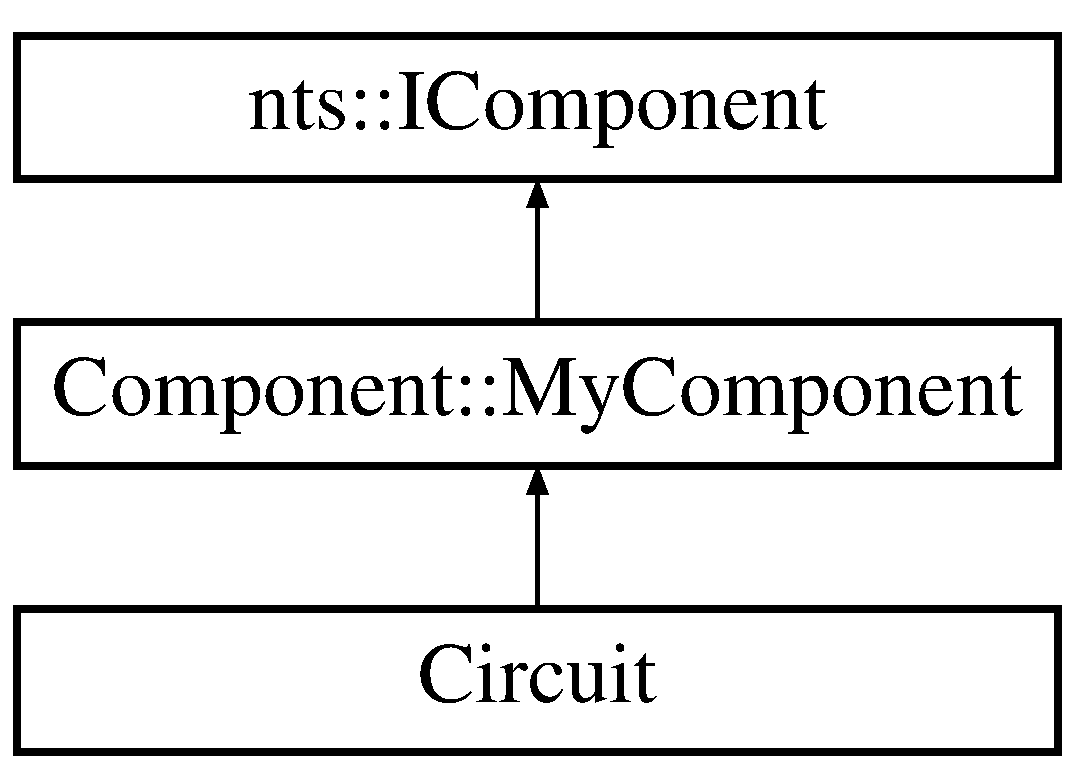
\includegraphics[height=3.000000cm]{classCircuit}
\end{center}
\end{figure}
\subsection*{Public Member Functions}
\begin{DoxyCompactItemize}
\item 
\mbox{\Hypertarget{classCircuit_ac3e4b6c48378994ee35289315eeb0951}\label{classCircuit_ac3e4b6c48378994ee35289315eeb0951}} 
void {\bfseries set\+Link} (std\+::size\+\_\+t pin, \mbox{\hyperlink{classnts_1_1IComponent}{nts\+::\+I\+Component}} \&other, std\+::size\+\_\+t other\+Pin)
\item 
\mbox{\Hypertarget{classCircuit_a7fdf649eb16d5d8f50b933f4ab7e3530}\label{classCircuit_a7fdf649eb16d5d8f50b933f4ab7e3530}} 
void {\bfseries set\+Input} (std\+::size\+\_\+t pin, \mbox{\hyperlink{classnts_1_1IComponent}{nts\+::\+I\+Component}} \&other, std\+::size\+\_\+t other\+Pin)
\item 
\mbox{\Hypertarget{classCircuit_a4cf8e76b22cc073499b5885dd11219a8}\label{classCircuit_a4cf8e76b22cc073499b5885dd11219a8}} 
void {\bfseries set\+Output} (std\+::size\+\_\+t pin, \mbox{\hyperlink{classnts_1_1IComponent}{nts\+::\+I\+Component}} \&other, std\+::size\+\_\+t other\+Pin)
\item 
\mbox{\Hypertarget{classCircuit_ace2804eb8778c9b2ec7f78eb1ac5ab38}\label{classCircuit_ace2804eb8778c9b2ec7f78eb1ac5ab38}} 
void {\bfseries create\+All\+Components} (const Parser\+::container\+\_\+setting\+\_\+t \&settings) final
\item 
\mbox{\Hypertarget{classCircuit_a6db179162b5e33f700d8509938c90c32}\label{classCircuit_a6db179162b5e33f700d8509938c90c32}} 
void {\bfseries set\+State} (const std\+::string \&name, const std\+::string \&state) final
\item 
\mbox{\Hypertarget{classCircuit_a737459bd18ae5b4bc73ff8a98c2241b6}\label{classCircuit_a737459bd18ae5b4bc73ff8a98c2241b6}} 
nts\+::\+Tristate {\bfseries compute} (std\+::size\+\_\+t) override
\item 
\mbox{\Hypertarget{classCircuit_a65d35a6e4080bea4aa8be011ae2ab04d}\label{classCircuit_a65d35a6e4080bea4aa8be011ae2ab04d}} 
void {\bfseries dump} () const noexcept override
\end{DoxyCompactItemize}
\subsection*{Additional Inherited Members}


The documentation for this class was generated from the following files\+:\begin{DoxyCompactItemize}
\item 
Include/Circuit.\+hpp\item 
Src/\+Components/Circuit.\+cpp\end{DoxyCompactItemize}

\hypertarget{structComponent_1_1ComponentSetting}{}\section{Component\+:\+:Component\+Setting Struct Reference}
\label{structComponent_1_1ComponentSetting}\index{Component\+::\+Component\+Setting@{Component\+::\+Component\+Setting}}
\subsection*{Public Attributes}
\begin{DoxyCompactItemize}
\item 
\mbox{\Hypertarget{structComponent_1_1ComponentSetting_aae5ad8d8f44adeb832d1cb1359835ead}\label{structComponent_1_1ComponentSetting_aae5ad8d8f44adeb832d1cb1359835ead}} 
std\+::string {\bfseries name}
\item 
\mbox{\Hypertarget{structComponent_1_1ComponentSetting_a694498bbd5915773b32ee1c0e702f496}\label{structComponent_1_1ComponentSetting_a694498bbd5915773b32ee1c0e702f496}} 
std\+::string {\bfseries value}
\item 
\mbox{\Hypertarget{structComponent_1_1ComponentSetting_a3545a3c79285d29ba412eed11fb8331a}\label{structComponent_1_1ComponentSetting_a3545a3c79285d29ba412eed11fb8331a}} 
nts\+::\+Type {\bfseries type}
\item 
\mbox{\Hypertarget{structComponent_1_1ComponentSetting_a935fc46bbed4216aab77ea7b27708e8f}\label{structComponent_1_1ComponentSetting_a935fc46bbed4216aab77ea7b27708e8f}} 
std\+::vector$<$ \mbox{\hyperlink{structComponent_1_1Link}{Link}} $>$ {\bfseries links}
\end{DoxyCompactItemize}


The documentation for this struct was generated from the following file\+:\begin{DoxyCompactItemize}
\item 
Include/Setting.\+hpp\end{DoxyCompactItemize}

\hypertarget{classError_1_1Component_1_1ComputeError}{}\section{Error\+:\+:Component\+:\+:Compute\+Error Class Reference}
\label{classError_1_1Component_1_1ComputeError}\index{Error\+::\+Component\+::\+Compute\+Error@{Error\+::\+Component\+::\+Compute\+Error}}
Inheritance diagram for Error\+:\+:Component\+:\+:Compute\+Error\+:\begin{figure}[H]
\begin{center}
\leavevmode
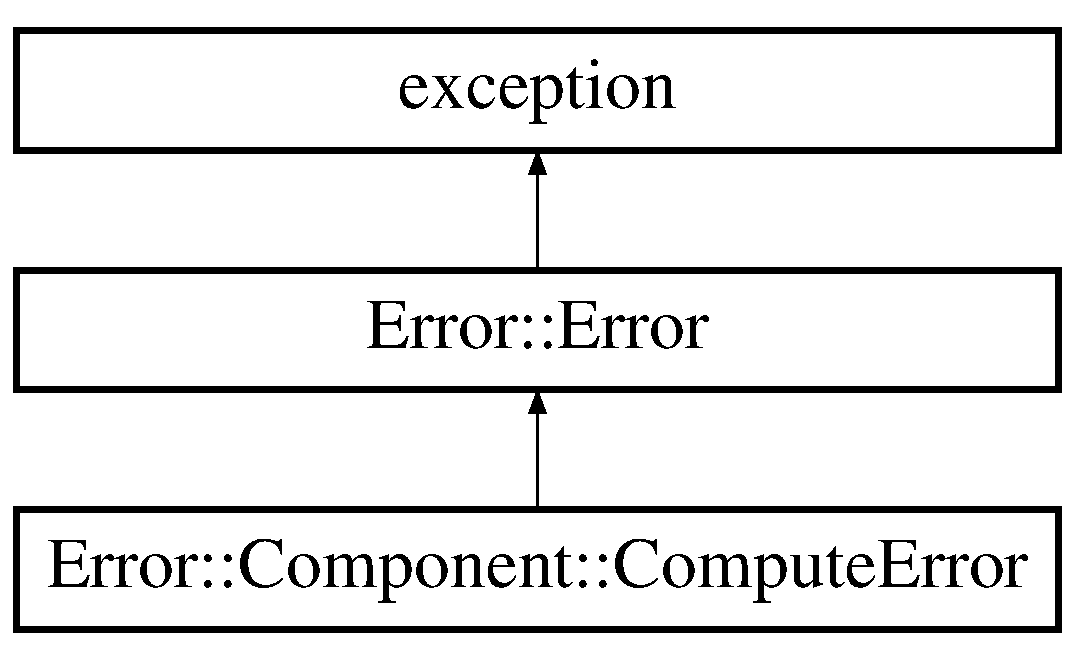
\includegraphics[height=3.000000cm]{classError_1_1Component_1_1ComputeError}
\end{center}
\end{figure}
\subsection*{Public Member Functions}
\begin{DoxyCompactItemize}
\item 
\mbox{\Hypertarget{classError_1_1Component_1_1ComputeError_ad206f30d8d4466ed8547a44f9d13868f}\label{classError_1_1Component_1_1ComputeError_ad206f30d8d4466ed8547a44f9d13868f}} 
{\bfseries Compute\+Error} (std\+::string const \&message, std\+::string const \&where=\char`\"{}Unknown\char`\"{})
\end{DoxyCompactItemize}
\subsection*{Additional Inherited Members}


The documentation for this class was generated from the following file\+:\begin{DoxyCompactItemize}
\item 
Include/Error.\+hpp\end{DoxyCompactItemize}

\hypertarget{classError_1_1Component_1_1CreationError}{}\section{Error\+:\+:Component\+:\+:Creation\+Error Class Reference}
\label{classError_1_1Component_1_1CreationError}\index{Error\+::\+Component\+::\+Creation\+Error@{Error\+::\+Component\+::\+Creation\+Error}}
Inheritance diagram for Error\+:\+:Component\+:\+:Creation\+Error\+:\begin{figure}[H]
\begin{center}
\leavevmode
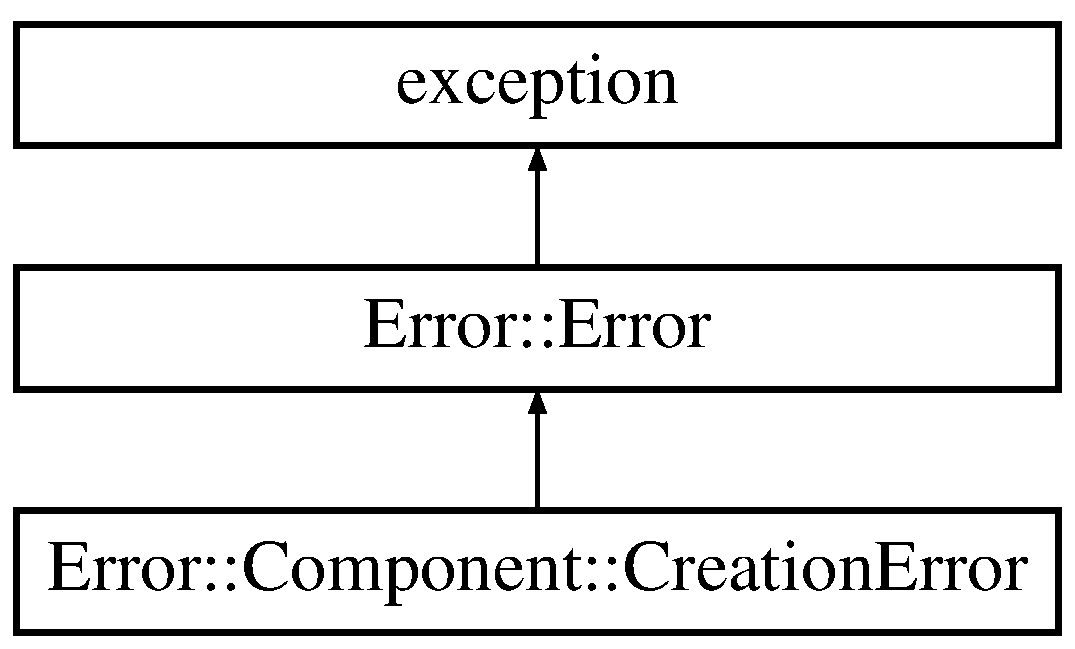
\includegraphics[height=3.000000cm]{classError_1_1Component_1_1CreationError}
\end{center}
\end{figure}
\subsection*{Public Member Functions}
\begin{DoxyCompactItemize}
\item 
\mbox{\Hypertarget{classError_1_1Component_1_1CreationError_ae30e73dab437659d6b2a27cb47efa130}\label{classError_1_1Component_1_1CreationError_ae30e73dab437659d6b2a27cb47efa130}} 
{\bfseries Creation\+Error} (std\+::string const \&message, std\+::string const \&where=\char`\"{}Unknown\char`\"{})
\end{DoxyCompactItemize}
\subsection*{Additional Inherited Members}


The documentation for this class was generated from the following file\+:\begin{DoxyCompactItemize}
\item 
Include/Error.\+hpp\end{DoxyCompactItemize}

\hypertarget{structnts_1_1Door}{}\section{nts\+:\+:Door Struct Reference}
\label{structnts_1_1Door}\index{nts\+::\+Door@{nts\+::\+Door}}
\subsection*{Public Attributes}
\begin{DoxyCompactItemize}
\item 
\mbox{\Hypertarget{structnts_1_1Door_a4d8b9c5416e7570afa88c65c5e6eeae3}\label{structnts_1_1Door_a4d8b9c5416e7570afa88c65c5e6eeae3}} 
\mbox{\hyperlink{structnts_1_1Pin}{nts\+::\+Pin}} {\bfseries input1}
\item 
\mbox{\Hypertarget{structnts_1_1Door_ac9f4f9247236b7df0ffb0a4f9925f563}\label{structnts_1_1Door_ac9f4f9247236b7df0ffb0a4f9925f563}} 
\mbox{\hyperlink{structnts_1_1Pin}{nts\+::\+Pin}} {\bfseries input2}
\item 
\mbox{\Hypertarget{structnts_1_1Door_a66d30c7a27c9f160d8ffd71cb7f5933f}\label{structnts_1_1Door_a66d30c7a27c9f160d8ffd71cb7f5933f}} 
\mbox{\hyperlink{structnts_1_1Pin}{nts\+::\+Pin}} {\bfseries output}
\end{DoxyCompactItemize}


The documentation for this struct was generated from the following file\+:\begin{DoxyCompactItemize}
\item 
Include/I\+Component.\+hpp\end{DoxyCompactItemize}

\hypertarget{classError_1_1Error}{}\section{Error\+:\+:Error Class Reference}
\label{classError_1_1Error}\index{Error\+::\+Error@{Error\+::\+Error}}
Inheritance diagram for Error\+:\+:Error\+:\begin{figure}[H]
\begin{center}
\leavevmode
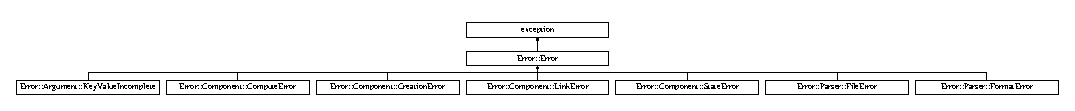
\includegraphics[height=1.038961cm]{classError_1_1Error}
\end{center}
\end{figure}
\subsection*{Public Member Functions}
\begin{DoxyCompactItemize}
\item 
\mbox{\Hypertarget{classError_1_1Error_a58b5a784c9b6ffd414ef23dfccdfd69d}\label{classError_1_1Error_a58b5a784c9b6ffd414ef23dfccdfd69d}} 
{\bfseries Error} (const std\+::string \&message, const std\+::string \&where=\char`\"{}Unknown\char`\"{})
\item 
\mbox{\Hypertarget{classError_1_1Error_ac760553ea2ad58d079155097a2853ac0}\label{classError_1_1Error_ac760553ea2ad58d079155097a2853ac0}} 
const std\+::string \& {\bfseries where} () const
\item 
\mbox{\Hypertarget{classError_1_1Error_aa9c29452b1555ad2c74c0aacb7cfef63}\label{classError_1_1Error_aa9c29452b1555ad2c74c0aacb7cfef63}} 
const char $\ast$ {\bfseries what} () const noexcept override
\end{DoxyCompactItemize}
\subsection*{Protected Attributes}
\begin{DoxyCompactItemize}
\item 
\mbox{\Hypertarget{classError_1_1Error_ade9c29db1fe508eccb653635ef058e68}\label{classError_1_1Error_ade9c29db1fe508eccb653635ef058e68}} 
std\+::string {\bfseries \+\_\+where}
\end{DoxyCompactItemize}


The documentation for this class was generated from the following files\+:\begin{DoxyCompactItemize}
\item 
Include/Error.\+hpp\item 
Src/Error.\+cpp\end{DoxyCompactItemize}

\hypertarget{classFactory}{}\section{Factory Class Reference}
\label{classFactory}\index{Factory@{Factory}}
\subsection*{Public Member Functions}
\begin{DoxyCompactItemize}
\item 
\mbox{\Hypertarget{classFactory_a79d88109234e117dbaf4c1a7815cf8d8}\label{classFactory_a79d88109234e117dbaf4c1a7815cf8d8}} 
std\+::unique\+\_\+ptr$<$ \mbox{\hyperlink{classnts_1_1IComponent}{nts\+::\+I\+Component}} $>$ {\bfseries create\+Component} (const nts\+::\+Type type, const std\+::string \&value)
\item 
\mbox{\Hypertarget{classFactory_a72b2647bfa6c5da1bc8cc3a43014ca69}\label{classFactory_a72b2647bfa6c5da1bc8cc3a43014ca69}} 
void {\bfseries link\+All\+Components} (std\+::map$<$ std\+::string, nts\+::ptr\+I\+Component\+\_\+t $>$ \&components, const std\+::vector$<$ \mbox{\hyperlink{structComponent_1_1ComponentSetting}{Component\+::\+Component\+Setting}} $>$ \&settings)
\end{DoxyCompactItemize}


The documentation for this class was generated from the following files\+:\begin{DoxyCompactItemize}
\item 
Include/Factory.\+hpp\item 
Src/\+Components/Factory.\+cpp\end{DoxyCompactItemize}

\hypertarget{classFalse}{}\section{False Class Reference}
\label{classFalse}\index{False@{False}}
Inheritance diagram for False\+:\begin{figure}[H]
\begin{center}
\leavevmode
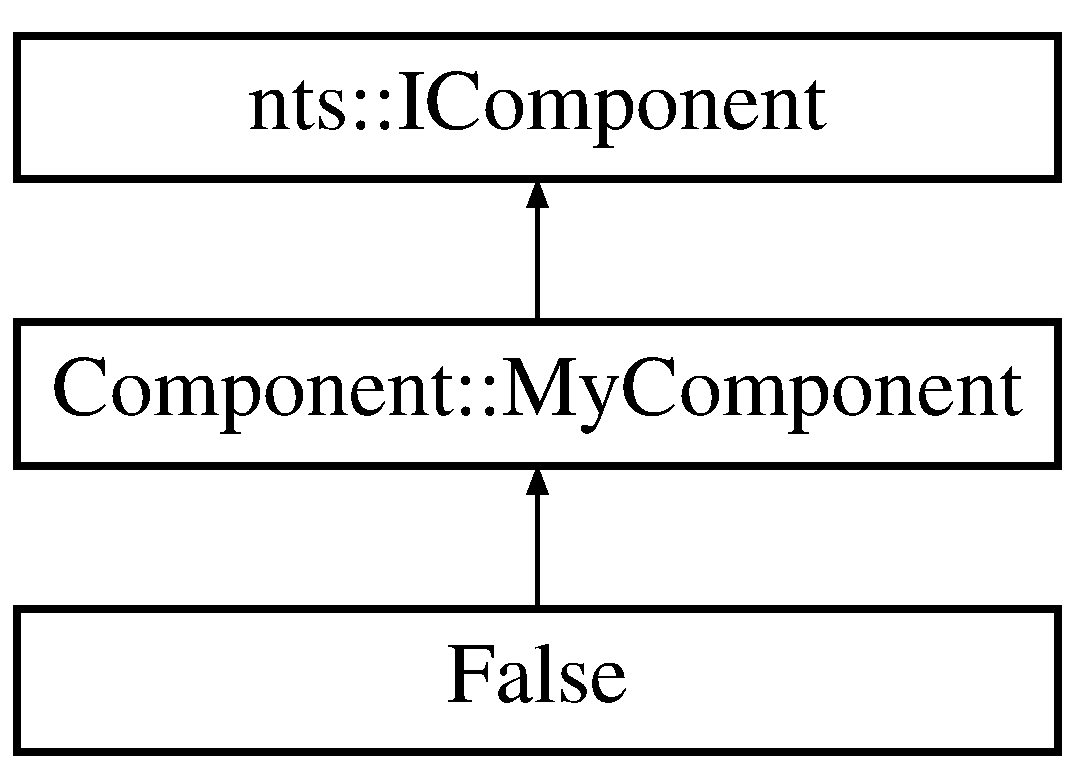
\includegraphics[height=3.000000cm]{classFalse}
\end{center}
\end{figure}
\subsection*{Public Member Functions}
\begin{DoxyCompactItemize}
\item 
\mbox{\Hypertarget{classFalse_a929c783787b5a1bc14840d851e294018}\label{classFalse_a929c783787b5a1bc14840d851e294018}} 
nts\+::\+Tristate {\bfseries compute} (std\+::size\+\_\+t pin=1) override
\item 
\mbox{\Hypertarget{classFalse_adcd692fb9aa96767996f95cebec02537}\label{classFalse_adcd692fb9aa96767996f95cebec02537}} 
void {\bfseries set\+Link} (std\+::size\+\_\+t pin, \mbox{\hyperlink{classnts_1_1IComponent}{nts\+::\+I\+Component}} \&other, std\+::size\+\_\+t other\+Pin) override
\item 
\mbox{\Hypertarget{classFalse_ab5fac5b173572ed8a544cc6f22b1801b}\label{classFalse_ab5fac5b173572ed8a544cc6f22b1801b}} 
void {\bfseries dump} () const noexcept override
\item 
\mbox{\Hypertarget{classFalse_aaaf87a7c14cda94fc240b82ce0d7ef59}\label{classFalse_aaaf87a7c14cda94fc240b82ce0d7ef59}} 
void {\bfseries set\+Input} (std\+::size\+\_\+t pin, \mbox{\hyperlink{classnts_1_1IComponent}{nts\+::\+I\+Component}} \&other, std\+::size\+\_\+t other\+Pin) final
\item 
\mbox{\Hypertarget{classFalse_ae3d9904440a2424999d3ad8406e54008}\label{classFalse_ae3d9904440a2424999d3ad8406e54008}} 
void {\bfseries set\+Output} (std\+::size\+\_\+t pin, \mbox{\hyperlink{classnts_1_1IComponent}{nts\+::\+I\+Component}} \&other, std\+::size\+\_\+t other\+Pin) final
\end{DoxyCompactItemize}
\subsection*{Additional Inherited Members}


The documentation for this class was generated from the following files\+:\begin{DoxyCompactItemize}
\item 
Include/False.\+hpp\item 
Src/\+Components/False.\+cpp\end{DoxyCompactItemize}

\hypertarget{classError_1_1Parser_1_1FileError}{}\section{Error\+:\+:Parser\+:\+:File\+Error Class Reference}
\label{classError_1_1Parser_1_1FileError}\index{Error\+::\+Parser\+::\+File\+Error@{Error\+::\+Parser\+::\+File\+Error}}
Inheritance diagram for Error\+:\+:Parser\+:\+:File\+Error\+:\begin{figure}[H]
\begin{center}
\leavevmode
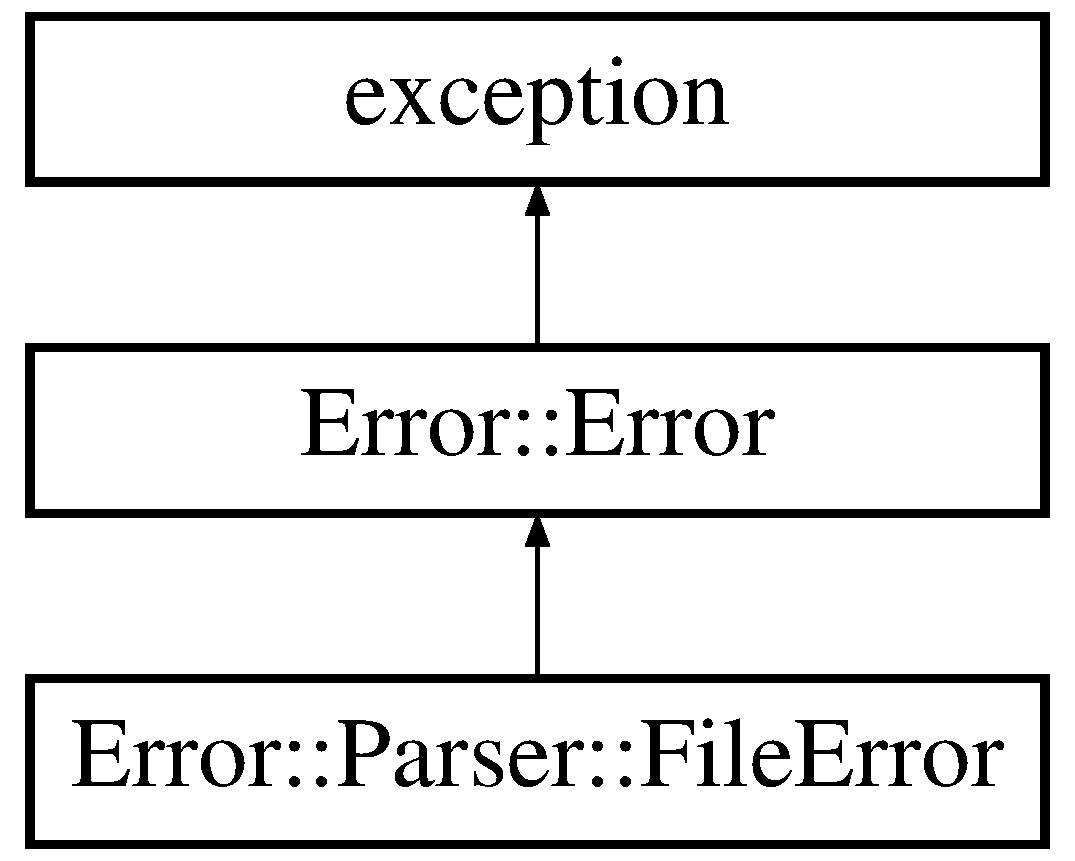
\includegraphics[height=3.000000cm]{classError_1_1Parser_1_1FileError}
\end{center}
\end{figure}
\subsection*{Public Member Functions}
\begin{DoxyCompactItemize}
\item 
\mbox{\Hypertarget{classError_1_1Parser_1_1FileError_af1ea2c413a42cd894245019510421481}\label{classError_1_1Parser_1_1FileError_af1ea2c413a42cd894245019510421481}} 
{\bfseries File\+Error} (std\+::string const \&message, std\+::string const \&where=\char`\"{}Unknown\char`\"{})
\end{DoxyCompactItemize}
\subsection*{Additional Inherited Members}


The documentation for this class was generated from the following file\+:\begin{DoxyCompactItemize}
\item 
Include/Error.\+hpp\end{DoxyCompactItemize}

\hypertarget{classError_1_1Parser_1_1FormatError}{}\section{Error\+:\+:Parser\+:\+:Format\+Error Class Reference}
\label{classError_1_1Parser_1_1FormatError}\index{Error\+::\+Parser\+::\+Format\+Error@{Error\+::\+Parser\+::\+Format\+Error}}
Inheritance diagram for Error\+:\+:Parser\+:\+:Format\+Error\+:\begin{figure}[H]
\begin{center}
\leavevmode
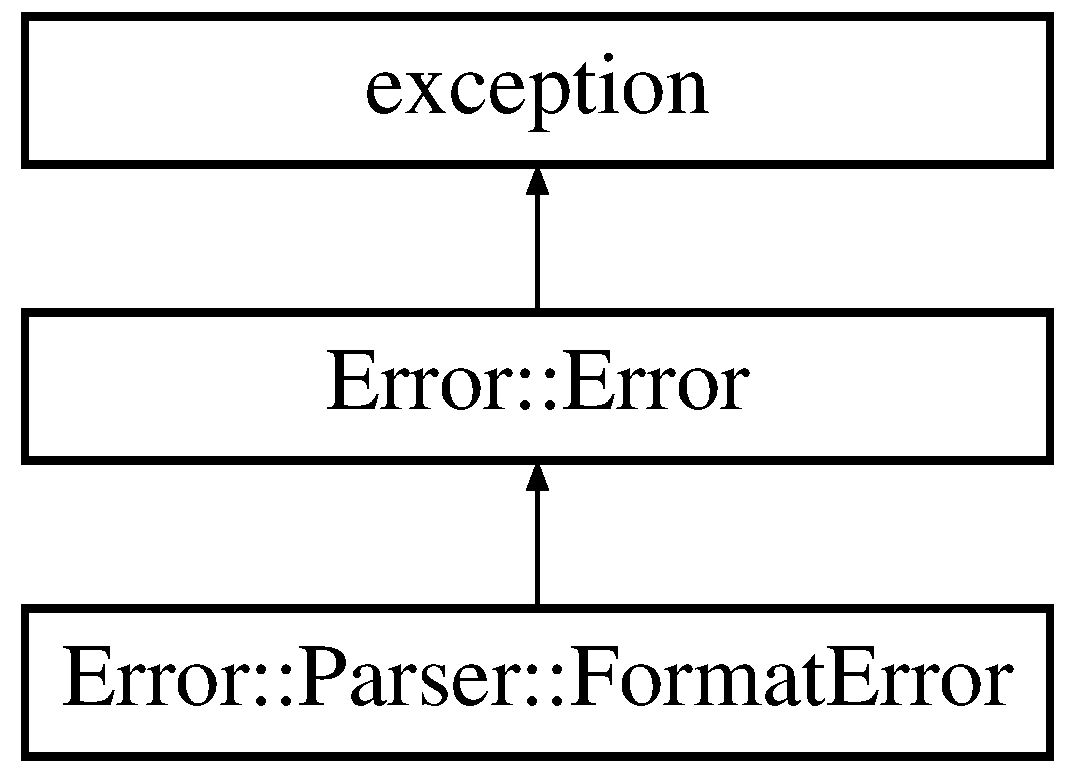
\includegraphics[height=3.000000cm]{classError_1_1Parser_1_1FormatError}
\end{center}
\end{figure}
\subsection*{Public Member Functions}
\begin{DoxyCompactItemize}
\item 
\mbox{\Hypertarget{classError_1_1Parser_1_1FormatError_ae27aad8b7c583d29d4bd40f23183034f}\label{classError_1_1Parser_1_1FormatError_ae27aad8b7c583d29d4bd40f23183034f}} 
{\bfseries Format\+Error} (std\+::string const \&message, std\+::string const \&where=\char`\"{}Unknown\char`\"{})
\end{DoxyCompactItemize}
\subsection*{Additional Inherited Members}


The documentation for this class was generated from the following file\+:\begin{DoxyCompactItemize}
\item 
Include/Error.\+hpp\end{DoxyCompactItemize}

\hypertarget{classnts_1_1IComponent}{}\section{nts\+:\+:I\+Component Class Reference}
\label{classnts_1_1IComponent}\index{nts\+::\+I\+Component@{nts\+::\+I\+Component}}
Inheritance diagram for nts\+:\+:I\+Component\+:\begin{figure}[H]
\begin{center}
\leavevmode
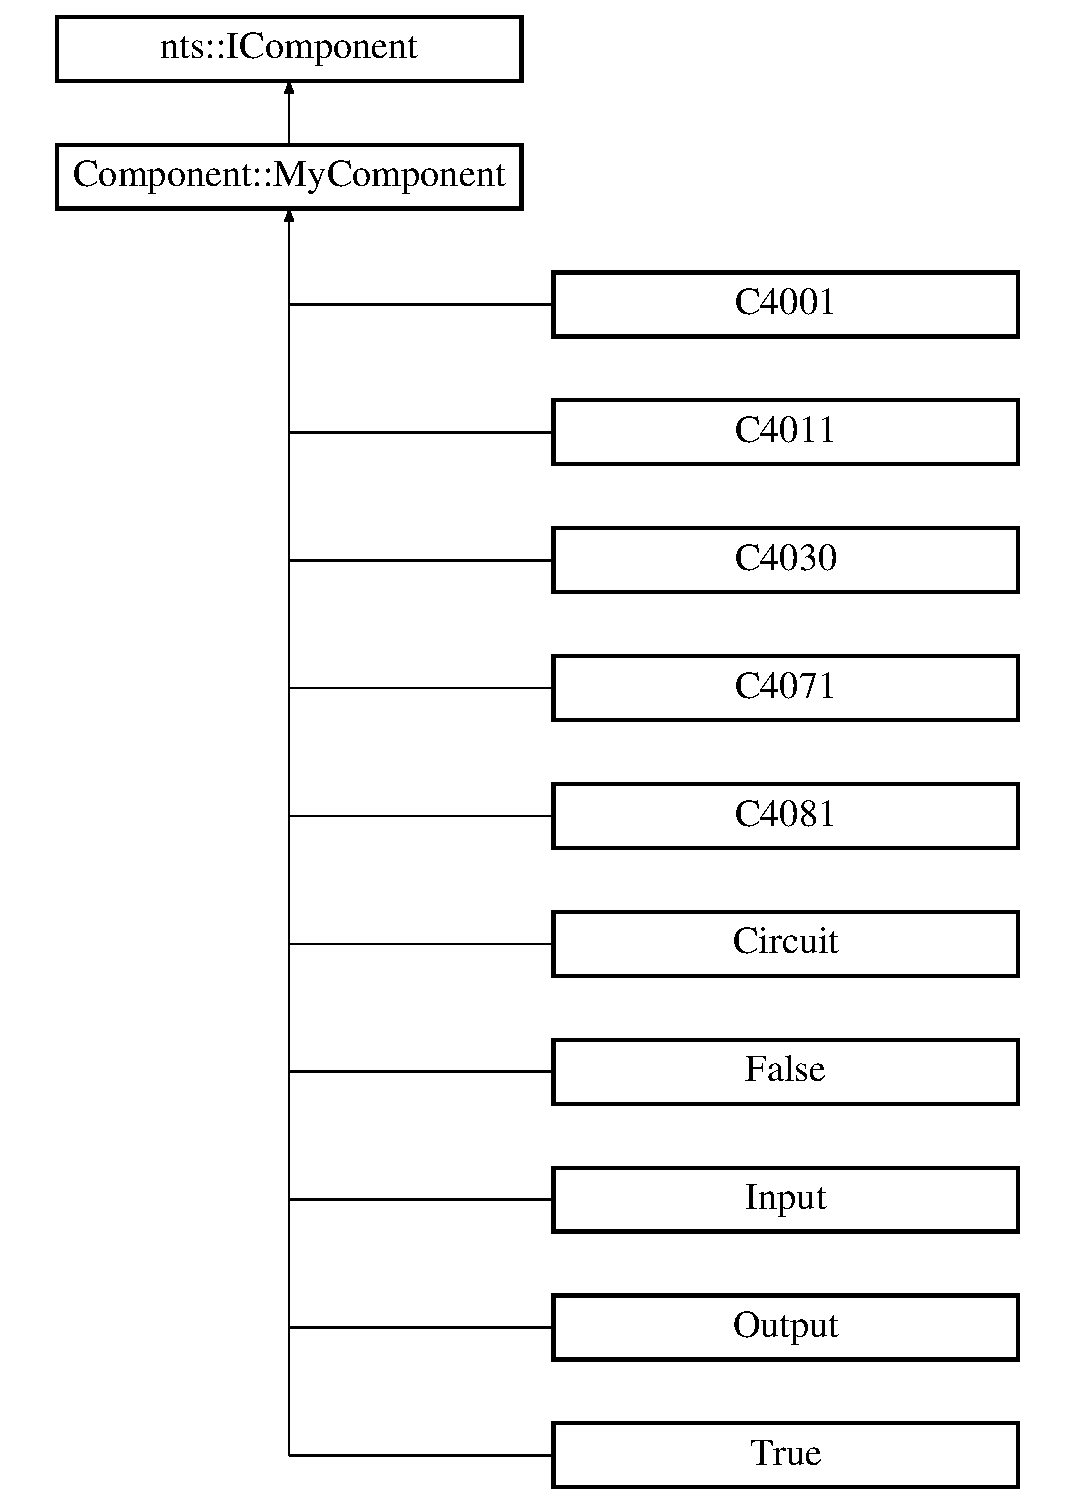
\includegraphics[height=12.000000cm]{classnts_1_1IComponent}
\end{center}
\end{figure}
\subsection*{Public Member Functions}
\begin{DoxyCompactItemize}
\item 
\mbox{\Hypertarget{classnts_1_1IComponent_a00158e91b34034cfc41902385f25da43}\label{classnts_1_1IComponent_a00158e91b34034cfc41902385f25da43}} 
virtual void {\bfseries create\+All\+Components} (const std\+::vector$<$ \mbox{\hyperlink{structComponent_1_1ComponentSetting}{Component\+::\+Component\+Setting}} $>$ \&settings)=0
\item 
\mbox{\Hypertarget{classnts_1_1IComponent_accdf4bbba897aa2315672f85600273d6}\label{classnts_1_1IComponent_accdf4bbba897aa2315672f85600273d6}} 
virtual nts\+::\+Tristate {\bfseries compute} (std\+::size\+\_\+t pin=1)=0
\item 
\mbox{\Hypertarget{classnts_1_1IComponent_a3208febc84b2056013b6d9ac6ed4a7d5}\label{classnts_1_1IComponent_a3208febc84b2056013b6d9ac6ed4a7d5}} 
virtual void {\bfseries set\+Link} (std\+::size\+\_\+t pin, \mbox{\hyperlink{classnts_1_1IComponent}{nts\+::\+I\+Component}} \&other, std\+::size\+\_\+t other\+Pin)=0
\item 
\mbox{\Hypertarget{classnts_1_1IComponent_abf1d98d16037a91b429798d4a1006516}\label{classnts_1_1IComponent_abf1d98d16037a91b429798d4a1006516}} 
virtual void {\bfseries dump} () const noexcept=0
\item 
\mbox{\Hypertarget{classnts_1_1IComponent_a09c9d36dbe8217e718e81a2c715bb8cf}\label{classnts_1_1IComponent_a09c9d36dbe8217e718e81a2c715bb8cf}} 
virtual void {\bfseries set\+Input} (std\+::size\+\_\+t pin, \mbox{\hyperlink{classnts_1_1IComponent}{nts\+::\+I\+Component}} \&other, std\+::size\+\_\+t other\+Pin)=0
\item 
\mbox{\Hypertarget{classnts_1_1IComponent_ab68b216d6ccb06b02e548d7a4a70a189}\label{classnts_1_1IComponent_ab68b216d6ccb06b02e548d7a4a70a189}} 
virtual void {\bfseries set\+Output} (std\+::size\+\_\+t pin, \mbox{\hyperlink{classnts_1_1IComponent}{nts\+::\+I\+Component}} \&other, std\+::size\+\_\+t other\+Pin)=0
\item 
\mbox{\Hypertarget{classnts_1_1IComponent_a73f8805b772a85bfefb826ceb0d233f3}\label{classnts_1_1IComponent_a73f8805b772a85bfefb826ceb0d233f3}} 
virtual void {\bfseries set\+State} (const std\+::string \&name, const std\+::string \&state)=0
\item 
\mbox{\Hypertarget{classnts_1_1IComponent_a688f0040fde588087f2db05b8127a9fb}\label{classnts_1_1IComponent_a688f0040fde588087f2db05b8127a9fb}} 
virtual void {\bfseries set\+State} (const std\+::string \&state)=0
\item 
\mbox{\Hypertarget{classnts_1_1IComponent_a61dfe7e130dee94f08b9aaca5a89be7e}\label{classnts_1_1IComponent_a61dfe7e130dee94f08b9aaca5a89be7e}} 
virtual void {\bfseries set\+Name} (const std\+::string \&name) noexcept=0
\item 
\mbox{\Hypertarget{classnts_1_1IComponent_ad9fece97a1cc1154953d9c0a9df7cab3}\label{classnts_1_1IComponent_ad9fece97a1cc1154953d9c0a9df7cab3}} 
virtual const std\+::string \& {\bfseries get\+Name} () const noexcept=0
\item 
\mbox{\Hypertarget{classnts_1_1IComponent_ac8050d5c0c2f6d4f426077d92b814c5d}\label{classnts_1_1IComponent_ac8050d5c0c2f6d4f426077d92b814c5d}} 
virtual const Type \& {\bfseries get\+Type} () const noexcept=0
\end{DoxyCompactItemize}


The documentation for this class was generated from the following file\+:\begin{DoxyCompactItemize}
\item 
Include/I\+Component.\+hpp\end{DoxyCompactItemize}

\hypertarget{classInput}{}\section{Input Class Reference}
\label{classInput}\index{Input@{Input}}
Inheritance diagram for Input\+:\begin{figure}[H]
\begin{center}
\leavevmode
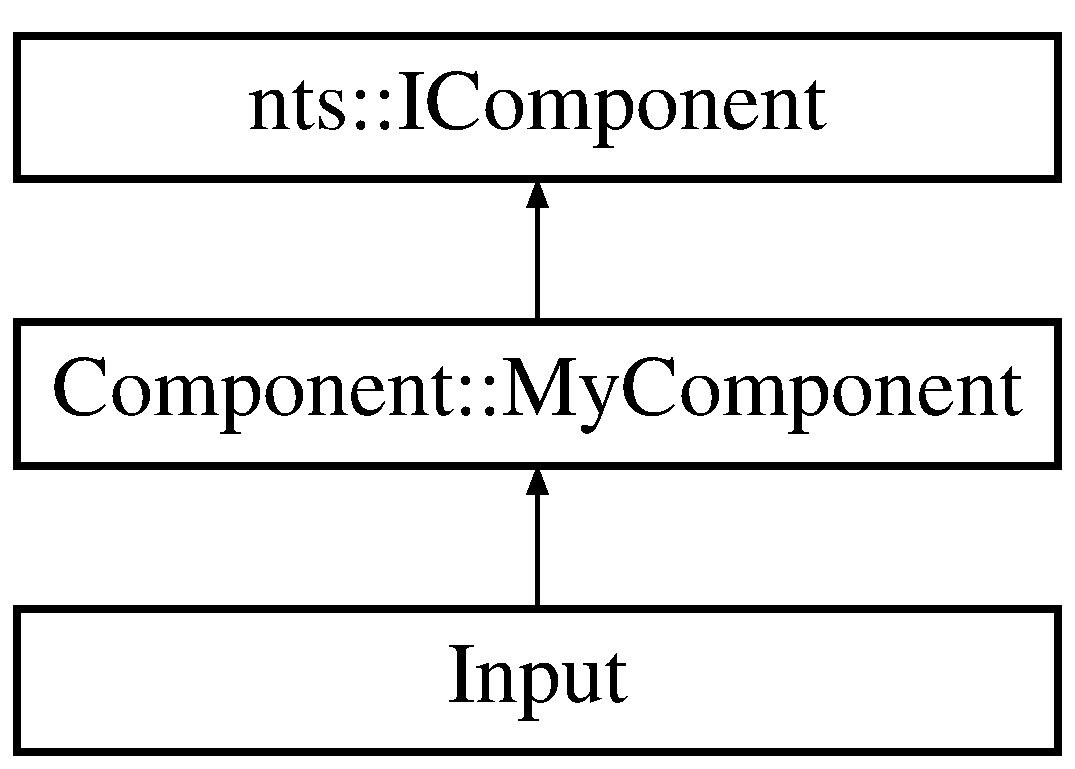
\includegraphics[height=3.000000cm]{classInput}
\end{center}
\end{figure}
\subsection*{Public Member Functions}
\begin{DoxyCompactItemize}
\item 
\mbox{\Hypertarget{classInput_a221cccaefc57a2f12e29e03878a15ab0}\label{classInput_a221cccaefc57a2f12e29e03878a15ab0}} 
nts\+::\+Tristate {\bfseries compute} (std\+::size\+\_\+t pin=1) override
\item 
\mbox{\Hypertarget{classInput_af680922e1c312e604586b3786d4bafa7}\label{classInput_af680922e1c312e604586b3786d4bafa7}} 
void {\bfseries set\+Link} (std\+::size\+\_\+t pin, \mbox{\hyperlink{classnts_1_1IComponent}{nts\+::\+I\+Component}} \&other, std\+::size\+\_\+t other\+Pin) override
\item 
\mbox{\Hypertarget{classInput_a6177d3295b4f81134ba3a8d643eacaf9}\label{classInput_a6177d3295b4f81134ba3a8d643eacaf9}} 
void {\bfseries dump} () const noexcept override
\item 
\mbox{\Hypertarget{classInput_a657e1fb517b93986e86112d83ca6514c}\label{classInput_a657e1fb517b93986e86112d83ca6514c}} 
void {\bfseries set\+Input} (std\+::size\+\_\+t pin, \mbox{\hyperlink{classnts_1_1IComponent}{nts\+::\+I\+Component}} \&other, std\+::size\+\_\+t other\+Pin) final
\item 
\mbox{\Hypertarget{classInput_a691d94760878e81c668c8e477aa17177}\label{classInput_a691d94760878e81c668c8e477aa17177}} 
void {\bfseries set\+Output} (std\+::size\+\_\+t pin, \mbox{\hyperlink{classnts_1_1IComponent}{nts\+::\+I\+Component}} \&other, std\+::size\+\_\+t other\+Pin) final
\item 
\mbox{\Hypertarget{classInput_a208afe1233da126674ef84ca4060ee56}\label{classInput_a208afe1233da126674ef84ca4060ee56}} 
void {\bfseries set\+State} (const std\+::string \&state) final
\end{DoxyCompactItemize}
\subsection*{Additional Inherited Members}


The documentation for this class was generated from the following files\+:\begin{DoxyCompactItemize}
\item 
Include/Input.\+hpp\item 
Src/\+Components/Input.\+cpp\end{DoxyCompactItemize}

\hypertarget{classError_1_1Argument_1_1KeyValueIncomplete}{}\section{Error\+:\+:Argument\+:\+:Key\+Value\+Incomplete Class Reference}
\label{classError_1_1Argument_1_1KeyValueIncomplete}\index{Error\+::\+Argument\+::\+Key\+Value\+Incomplete@{Error\+::\+Argument\+::\+Key\+Value\+Incomplete}}
Inheritance diagram for Error\+:\+:Argument\+:\+:Key\+Value\+Incomplete\+:\begin{figure}[H]
\begin{center}
\leavevmode
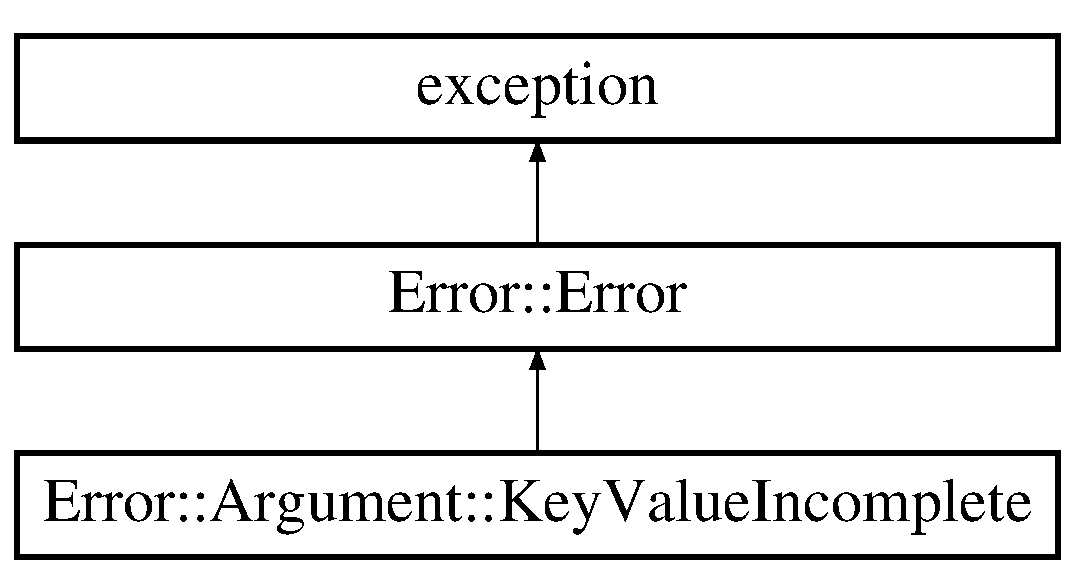
\includegraphics[height=3.000000cm]{classError_1_1Argument_1_1KeyValueIncomplete}
\end{center}
\end{figure}
\subsection*{Public Member Functions}
\begin{DoxyCompactItemize}
\item 
\mbox{\Hypertarget{classError_1_1Argument_1_1KeyValueIncomplete_a58e023982f3fce22da79f25fdabf1307}\label{classError_1_1Argument_1_1KeyValueIncomplete_a58e023982f3fce22da79f25fdabf1307}} 
{\bfseries Key\+Value\+Incomplete} (std\+::string const \&message, std\+::string const \&where=\char`\"{}Unknown\char`\"{})
\end{DoxyCompactItemize}
\subsection*{Additional Inherited Members}


The documentation for this class was generated from the following file\+:\begin{DoxyCompactItemize}
\item 
Include/Error.\+hpp\end{DoxyCompactItemize}

\hypertarget{classParser_1_1LineParser}{}\section{Parser\+:\+:Line\+Parser Class Reference}
\label{classParser_1_1LineParser}\index{Parser\+::\+Line\+Parser@{Parser\+::\+Line\+Parser}}
\subsection*{Public Member Functions}
\begin{DoxyCompactItemize}
\item 
\mbox{\Hypertarget{classParser_1_1LineParser_aad39093a5159f39ba24e7e2afc545b4e}\label{classParser_1_1LineParser_aad39093a5159f39ba24e7e2afc545b4e}} 
{\bfseries Line\+Parser} (const std\+::string \&line)
\item 
\mbox{\Hypertarget{classParser_1_1LineParser_af4f166941b0542889a9d74fbaf45026e}\label{classParser_1_1LineParser_af4f166941b0542889a9d74fbaf45026e}} 
const std\+::string \& {\bfseries Get\+Line} () const
\item 
\mbox{\Hypertarget{classParser_1_1LineParser_aa84201ccd9d42805185b6e522fed5e34}\label{classParser_1_1LineParser_aa84201ccd9d42805185b6e522fed5e34}} 
void {\bfseries Clear\+Line} ()
\item 
\mbox{\Hypertarget{classParser_1_1LineParser_a8d81c69e2fecbbecf10cba4b08611444}\label{classParser_1_1LineParser_a8d81c69e2fecbbecf10cba4b08611444}} 
void {\bfseries Remove\+Comment} ()
\item 
\mbox{\Hypertarget{classParser_1_1LineParser_aeaa42d570c8d05637f35e8c3fc73cae0}\label{classParser_1_1LineParser_aeaa42d570c8d05637f35e8c3fc73cae0}} 
nts\+::\+Type {\bfseries Get\+Type} (const std\+::string \&type\+Str) const
\item 
\mbox{\Hypertarget{classParser_1_1LineParser_a8e6b1842ab6c3279301f92689f103a82}\label{classParser_1_1LineParser_a8e6b1842ab6c3279301f92689f103a82}} 
\mbox{\hyperlink{structComponent_1_1ComponentSetting}{Component\+::\+Component\+Setting}} {\bfseries Get\+Info\+Component} () const
\item 
\mbox{\Hypertarget{classParser_1_1LineParser_a22403bad1a0cda0e45b9cd44bab7d52c}\label{classParser_1_1LineParser_a22403bad1a0cda0e45b9cd44bab7d52c}} 
\mbox{\hyperlink{structComponent_1_1Link}{Component\+::\+Link}} {\bfseries Get\+Link} () const
\item 
\mbox{\Hypertarget{classParser_1_1LineParser_a65ac673bada1929cf2839d787ee36353}\label{classParser_1_1LineParser_a65ac673bada1929cf2839d787ee36353}} 
std\+::map$<$ std\+::string, std\+::string $>$ {\bfseries Split\+Line\+In\+Two} () const
\end{DoxyCompactItemize}


The documentation for this class was generated from the following files\+:\begin{DoxyCompactItemize}
\item 
Include/Parser.\+hpp\item 
Src/\+Parser/Line\+Parser.\+cpp\end{DoxyCompactItemize}

\hypertarget{structComponent_1_1Link}{}\section{Component\+:\+:Link Struct Reference}
\label{structComponent_1_1Link}\index{Component\+::\+Link@{Component\+::\+Link}}
\subsection*{Public Attributes}
\begin{DoxyCompactItemize}
\item 
\mbox{\Hypertarget{structComponent_1_1Link_accffc50390a67907efb220216015f722}\label{structComponent_1_1Link_accffc50390a67907efb220216015f722}} 
std\+::string {\bfseries origin\+Name}
\item 
\mbox{\Hypertarget{structComponent_1_1Link_a5f908953b3647fec16089d77d8dcde77}\label{structComponent_1_1Link_a5f908953b3647fec16089d77d8dcde77}} 
int {\bfseries origin\+Pin}
\item 
\mbox{\Hypertarget{structComponent_1_1Link_a200f1974ba4ae45e0bb944072f787239}\label{structComponent_1_1Link_a200f1974ba4ae45e0bb944072f787239}} 
std\+::string {\bfseries destination\+Name}
\item 
\mbox{\Hypertarget{structComponent_1_1Link_a1042e582b5c3e7163b1b7c9a626c3d8f}\label{structComponent_1_1Link_a1042e582b5c3e7163b1b7c9a626c3d8f}} 
int {\bfseries destination\+Pin}
\end{DoxyCompactItemize}


The documentation for this struct was generated from the following file\+:\begin{DoxyCompactItemize}
\item 
Include/Setting.\+hpp\end{DoxyCompactItemize}

\hypertarget{classError_1_1Component_1_1LinkError}{}\section{Error\+:\+:Component\+:\+:Link\+Error Class Reference}
\label{classError_1_1Component_1_1LinkError}\index{Error\+::\+Component\+::\+Link\+Error@{Error\+::\+Component\+::\+Link\+Error}}
Inheritance diagram for Error\+:\+:Component\+:\+:Link\+Error\+:\begin{figure}[H]
\begin{center}
\leavevmode
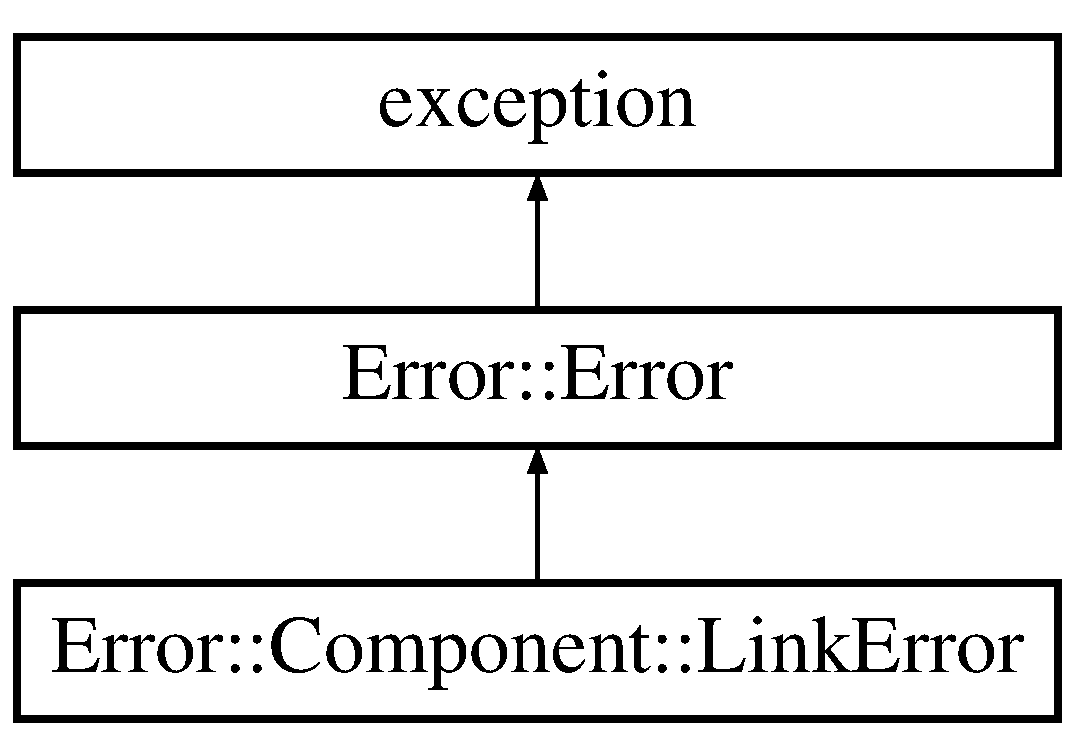
\includegraphics[height=3.000000cm]{classError_1_1Component_1_1LinkError}
\end{center}
\end{figure}
\subsection*{Public Member Functions}
\begin{DoxyCompactItemize}
\item 
\mbox{\Hypertarget{classError_1_1Component_1_1LinkError_a99177f7cad093b2351f057ce2c64b45b}\label{classError_1_1Component_1_1LinkError_a99177f7cad093b2351f057ce2c64b45b}} 
{\bfseries Link\+Error} (std\+::string const \&message, std\+::string const \&where=\char`\"{}Unknown\char`\"{})
\end{DoxyCompactItemize}
\subsection*{Additional Inherited Members}


The documentation for this class was generated from the following file\+:\begin{DoxyCompactItemize}
\item 
Include/Error.\+hpp\end{DoxyCompactItemize}

\hypertarget{classComponent_1_1MyComponent}{}\section{Component\+:\+:My\+Component Class Reference}
\label{classComponent_1_1MyComponent}\index{Component\+::\+My\+Component@{Component\+::\+My\+Component}}
Inheritance diagram for Component\+:\+:My\+Component\+:\begin{figure}[H]
\begin{center}
\leavevmode
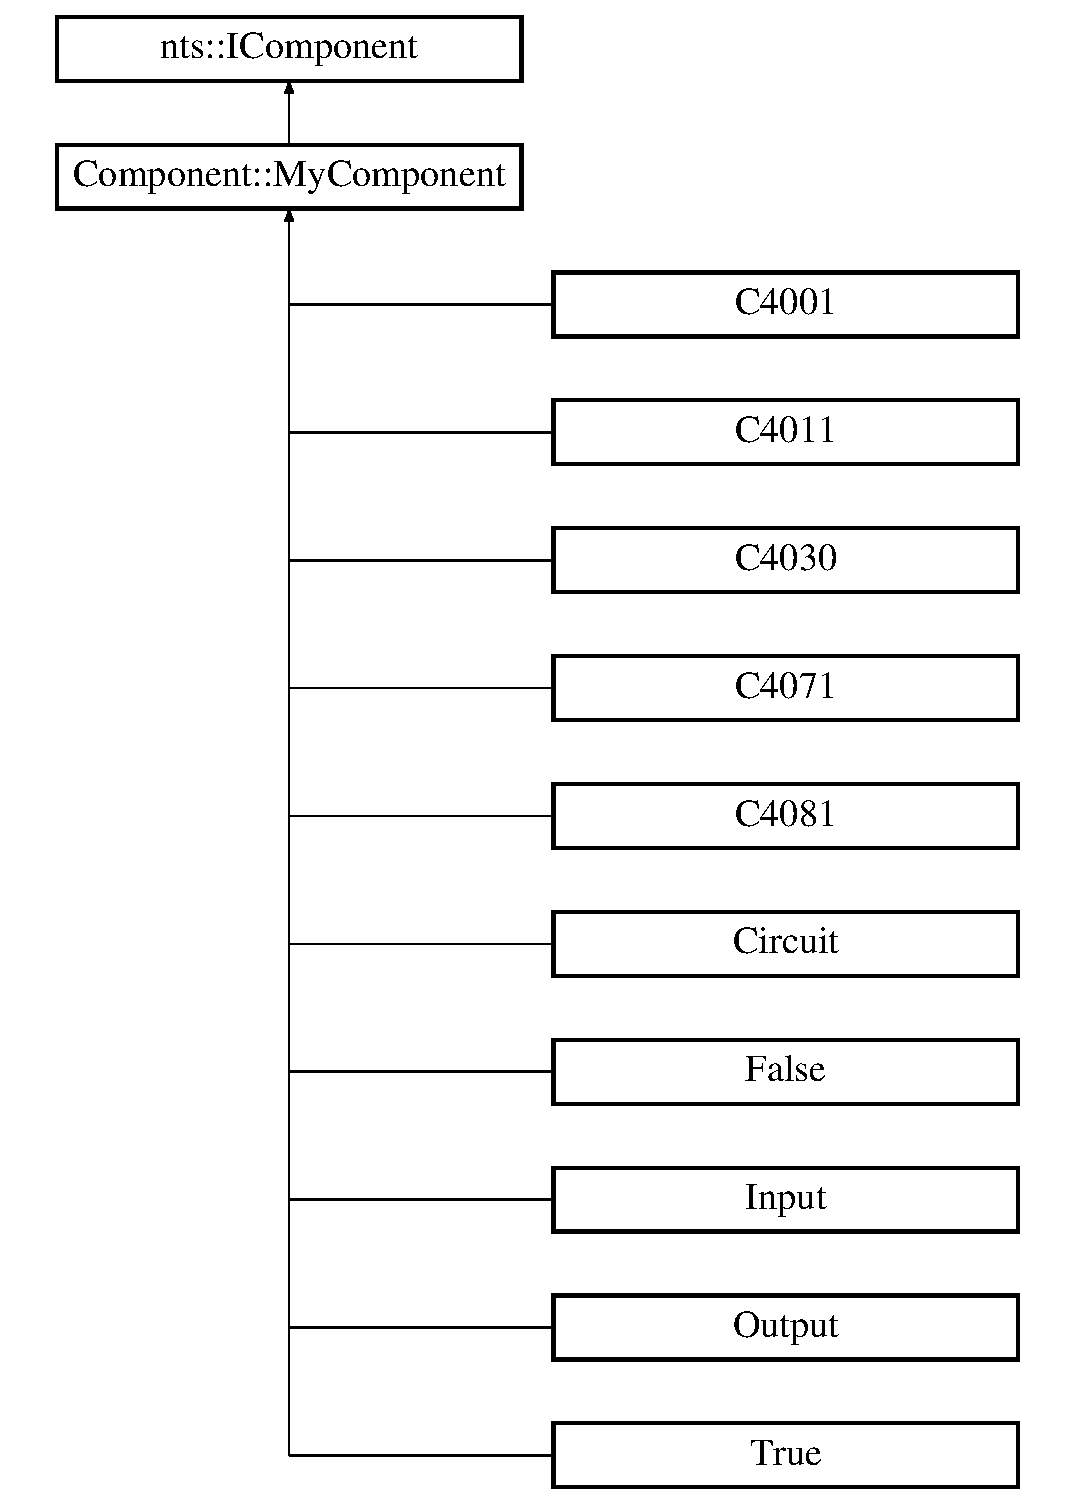
\includegraphics[height=12.000000cm]{classComponent_1_1MyComponent}
\end{center}
\end{figure}
\subsection*{Public Member Functions}
\begin{DoxyCompactItemize}
\item 
\mbox{\Hypertarget{classComponent_1_1MyComponent_a354699ef15d0a9dc1a8b85baf9e6179d}\label{classComponent_1_1MyComponent_a354699ef15d0a9dc1a8b85baf9e6179d}} 
{\bfseries My\+Component} (const nts\+::\+Type \&type)
\item 
\mbox{\Hypertarget{classComponent_1_1MyComponent_ad484b4bed8eed2723095311bdf431a83}\label{classComponent_1_1MyComponent_ad484b4bed8eed2723095311bdf431a83}} 
void {\bfseries create\+All\+Components} (const std\+::vector$<$ \mbox{\hyperlink{structComponent_1_1ComponentSetting}{Component\+::\+Component\+Setting}} $>$ \&settings)
\item 
\mbox{\Hypertarget{classComponent_1_1MyComponent_a1783b36ed6c0f02c232ad10d4ab0dc0d}\label{classComponent_1_1MyComponent_a1783b36ed6c0f02c232ad10d4ab0dc0d}} 
virtual void {\bfseries set\+State} (const std\+::string \&state)
\item 
\mbox{\Hypertarget{classComponent_1_1MyComponent_aa76da44b713bd627e239de4fff41c526}\label{classComponent_1_1MyComponent_aa76da44b713bd627e239de4fff41c526}} 
virtual void {\bfseries set\+State} (const std\+::string \&name, const std\+::string \&state)
\item 
\mbox{\Hypertarget{classComponent_1_1MyComponent_a632744b7989cfad5eab18a8b41cb9d3a}\label{classComponent_1_1MyComponent_a632744b7989cfad5eab18a8b41cb9d3a}} 
const std\+::string \& {\bfseries get\+Name} () const noexcept final
\item 
\mbox{\Hypertarget{classComponent_1_1MyComponent_a517586ccab356be9b4398fba050dcf38}\label{classComponent_1_1MyComponent_a517586ccab356be9b4398fba050dcf38}} 
void {\bfseries set\+Name} (const std\+::string \&name) noexcept final
\item 
\mbox{\Hypertarget{classComponent_1_1MyComponent_a9848edcd43b45bf4b00a54858b5d3f01}\label{classComponent_1_1MyComponent_a9848edcd43b45bf4b00a54858b5d3f01}} 
const nts\+::\+Type \& {\bfseries get\+Type} () const noexcept final
\end{DoxyCompactItemize}
\subsection*{Protected Attributes}
\begin{DoxyCompactItemize}
\item 
\mbox{\Hypertarget{classComponent_1_1MyComponent_ad8bdf4875c9b38b8f993d0d8b2b061ed}\label{classComponent_1_1MyComponent_ad8bdf4875c9b38b8f993d0d8b2b061ed}} 
std\+::string {\bfseries \+\_\+name}
\item 
\mbox{\Hypertarget{classComponent_1_1MyComponent_a97b7442dac976e6f1d64e95636e5a2b4}\label{classComponent_1_1MyComponent_a97b7442dac976e6f1d64e95636e5a2b4}} 
nts\+::\+Type {\bfseries \+\_\+type}
\end{DoxyCompactItemize}


The documentation for this class was generated from the following files\+:\begin{DoxyCompactItemize}
\item 
Include/Component.\+hpp\item 
Src/\+Components/Component.\+cpp\end{DoxyCompactItemize}

\hypertarget{classOutput}{}\section{Output Class Reference}
\label{classOutput}\index{Output@{Output}}
Inheritance diagram for Output\+:\begin{figure}[H]
\begin{center}
\leavevmode
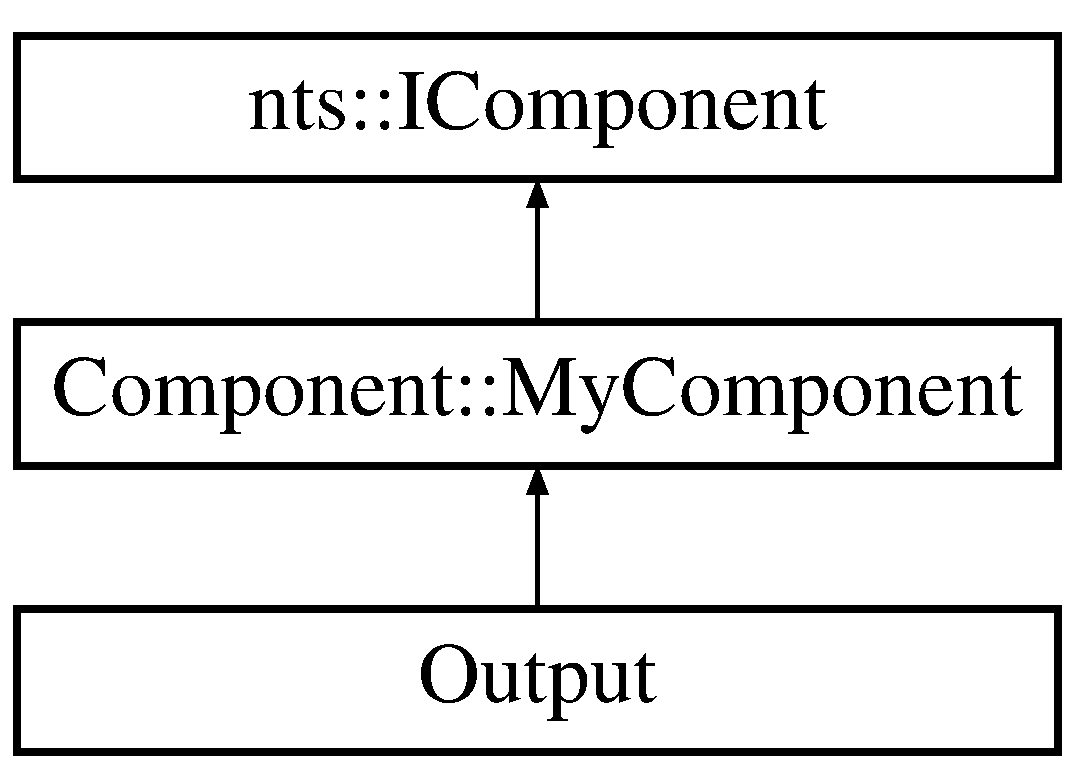
\includegraphics[height=3.000000cm]{classOutput}
\end{center}
\end{figure}
\subsection*{Public Member Functions}
\begin{DoxyCompactItemize}
\item 
\mbox{\Hypertarget{classOutput_a52cad797fc38f633476965aa7907fd21}\label{classOutput_a52cad797fc38f633476965aa7907fd21}} 
nts\+::\+Tristate {\bfseries compute} (std\+::size\+\_\+t pin=1) override
\item 
\mbox{\Hypertarget{classOutput_a3b109a0a1422e178af7e4571aecf347e}\label{classOutput_a3b109a0a1422e178af7e4571aecf347e}} 
void {\bfseries set\+Link} (std\+::size\+\_\+t pin, \mbox{\hyperlink{classnts_1_1IComponent}{nts\+::\+I\+Component}} \&other, std\+::size\+\_\+t other\+Pin) override
\item 
\mbox{\Hypertarget{classOutput_a4518c94c7c9e75704e5ea6b8a561588e}\label{classOutput_a4518c94c7c9e75704e5ea6b8a561588e}} 
void {\bfseries dump} () const noexcept override
\item 
\mbox{\Hypertarget{classOutput_ae981486010e5fe39b5a1bb369968827d}\label{classOutput_ae981486010e5fe39b5a1bb369968827d}} 
void {\bfseries set\+Input} (std\+::size\+\_\+t pin, \mbox{\hyperlink{classnts_1_1IComponent}{nts\+::\+I\+Component}} \&other, std\+::size\+\_\+t other\+Pin) final
\item 
\mbox{\Hypertarget{classOutput_a91d2273bcd7a7989d76e0f07960655c4}\label{classOutput_a91d2273bcd7a7989d76e0f07960655c4}} 
void {\bfseries set\+Output} (std\+::size\+\_\+t pin, \mbox{\hyperlink{classnts_1_1IComponent}{nts\+::\+I\+Component}} \&other, std\+::size\+\_\+t other\+Pin) final
\end{DoxyCompactItemize}
\subsection*{Additional Inherited Members}


The documentation for this class was generated from the following files\+:\begin{DoxyCompactItemize}
\item 
Include/Output.\+hpp\item 
Src/\+Components/Output.\+cpp\end{DoxyCompactItemize}

\hypertarget{classParser_1_1Parser}{}\section{Parser\+:\+:Parser Class Reference}
\label{classParser_1_1Parser}\index{Parser\+::\+Parser@{Parser\+::\+Parser}}
\subsection*{Public Member Functions}
\begin{DoxyCompactItemize}
\item 
\mbox{\Hypertarget{classParser_1_1Parser_a952924a6b78b1c2578e50195578083df}\label{classParser_1_1Parser_a952924a6b78b1c2578e50195578083df}} 
{\bfseries Parser} (const std\+::string \&filename)
\item 
\mbox{\Hypertarget{classParser_1_1Parser_a2fd87731d739eac280d971d7ed5c92f8}\label{classParser_1_1Parser_a2fd87731d739eac280d971d7ed5c92f8}} 
const container\+\_\+setting\+\_\+t {\bfseries Parse} ()
\item 
\mbox{\Hypertarget{classParser_1_1Parser_a8424e2cb688b08587365d0b8fad5785c}\label{classParser_1_1Parser_a8424e2cb688b08587365d0b8fad5785c}} 
void {\bfseries Read\+File} ()
\item 
\mbox{\Hypertarget{classParser_1_1Parser_a9083391260511c55c4dd45a7da45a430}\label{classParser_1_1Parser_a9083391260511c55c4dd45a7da45a430}} 
std\+::ifstream {\bfseries Open\+File} () const
\item 
\mbox{\Hypertarget{classParser_1_1Parser_a02621eeb00222237d79ecdd99cd90155}\label{classParser_1_1Parser_a02621eeb00222237d79ecdd99cd90155}} 
void {\bfseries Add\+Links\+To\+Chipset\+Info} (const container\+\_\+link\+\_\+t \&all\+Links, container\+\_\+setting\+\_\+t \&components)
\item 
\mbox{\Hypertarget{classParser_1_1Parser_ad603df97da7d3d1df24ac9214d2d3b84}\label{classParser_1_1Parser_ad603df97da7d3d1df24ac9214d2d3b84}} 
void {\bfseries Handle\+Chipsets} (unsigned int \&i, container\+\_\+setting\+\_\+t \&ret)
\item 
\mbox{\Hypertarget{classParser_1_1Parser_a8e8336c488a8406630d997617cc4c617}\label{classParser_1_1Parser_a8e8336c488a8406630d997617cc4c617}} 
void {\bfseries Handle\+Links} (unsigned int \&i, container\+\_\+link\+\_\+t \&all\+Links)
\end{DoxyCompactItemize}


The documentation for this class was generated from the following files\+:\begin{DoxyCompactItemize}
\item 
Include/Parser.\+hpp\item 
Src/\+Parser/Parser.\+cpp\end{DoxyCompactItemize}

\hypertarget{structnts_1_1Pin}{}\section{nts\+:\+:Pin Struct Reference}
\label{structnts_1_1Pin}\index{nts\+::\+Pin@{nts\+::\+Pin}}
\subsection*{Public Attributes}
\begin{DoxyCompactItemize}
\item 
\mbox{\Hypertarget{structnts_1_1Pin_a56bb48d55a0e6d822f6260d107cb54ba}\label{structnts_1_1Pin_a56bb48d55a0e6d822f6260d107cb54ba}} 
size\+\_\+t {\bfseries pin}
\item 
\mbox{\Hypertarget{structnts_1_1Pin_a0a84d871606d7f334bee3ff83c265890}\label{structnts_1_1Pin_a0a84d871606d7f334bee3ff83c265890}} 
nts\+::\+Tristate {\bfseries state}
\item 
\mbox{\Hypertarget{structnts_1_1Pin_a41da0646d485e2482cefc5b399c781d8}\label{structnts_1_1Pin_a41da0646d485e2482cefc5b399c781d8}} 
\mbox{\hyperlink{classnts_1_1IComponent}{nts\+::\+I\+Component}} $\ast$ {\bfseries destination\+Name}
\item 
\mbox{\Hypertarget{structnts_1_1Pin_a198cbbf53016027c3352d4150895e7d7}\label{structnts_1_1Pin_a198cbbf53016027c3352d4150895e7d7}} 
int {\bfseries destination\+Pin}
\end{DoxyCompactItemize}


The documentation for this struct was generated from the following file\+:\begin{DoxyCompactItemize}
\item 
Include/I\+Component.\+hpp\end{DoxyCompactItemize}

\hypertarget{classSimulation_1_1Simulation}{}\section{Simulation\+:\+:Simulation Class Reference}
\label{classSimulation_1_1Simulation}\index{Simulation\+::\+Simulation@{Simulation\+::\+Simulation}}
\subsection*{Public Member Functions}
\begin{DoxyCompactItemize}
\item 
\mbox{\Hypertarget{classSimulation_1_1Simulation_a76f716557481fa87591764fe127ba0c4}\label{classSimulation_1_1Simulation_a76f716557481fa87591764fe127ba0c4}} 
void {\bfseries Run} ()
\item 
\mbox{\Hypertarget{classSimulation_1_1Simulation_aadcb620861a93109fbf78e7594f565ef}\label{classSimulation_1_1Simulation_aadcb620861a93109fbf78e7594f565ef}} 
void {\bfseries Display\+Prompt} () const
\item 
\mbox{\Hypertarget{classSimulation_1_1Simulation_a8219e53e9cb91d46c978333510acc41b}\label{classSimulation_1_1Simulation_a8219e53e9cb91d46c978333510acc41b}} 
void {\bfseries Get\+Action} ()
\item 
\mbox{\Hypertarget{classSimulation_1_1Simulation_ac967c92d37ff3e7cdf9ff175b0eaef38}\label{classSimulation_1_1Simulation_ac967c92d37ff3e7cdf9ff175b0eaef38}} 
void {\bfseries Analyse\+Action} ()
\item 
\mbox{\Hypertarget{classSimulation_1_1Simulation_a8f58b7b50246da7c6cf4b256346b47de}\label{classSimulation_1_1Simulation_a8f58b7b50246da7c6cf4b256346b47de}} 
void {\bfseries create\+Circuit} (const Parser\+::container\+\_\+setting\+\_\+t \&settings)
\item 
\mbox{\Hypertarget{classSimulation_1_1Simulation_aba2a9d7d14c5a38749c85ba344f9a208}\label{classSimulation_1_1Simulation_aba2a9d7d14c5a38749c85ba344f9a208}} 
void {\bfseries set\+States} (const std\+::map$<$ std\+::string, std\+::string $>$ \&input\+Values)
\item 
\mbox{\Hypertarget{classSimulation_1_1Simulation_a8db10dc7a246e985fd1a1deb8b05f29f}\label{classSimulation_1_1Simulation_a8db10dc7a246e985fd1a1deb8b05f29f}} 
void {\bfseries simulate} ()
\item 
\mbox{\Hypertarget{classSimulation_1_1Simulation_aed2302b1ff4d372c2c8b60f7d633a185}\label{classSimulation_1_1Simulation_aed2302b1ff4d372c2c8b60f7d633a185}} 
void {\bfseries dump} () const noexcept
\item 
\mbox{\Hypertarget{classSimulation_1_1Simulation_a2efb3584b9bae48773cf65b88e131c87}\label{classSimulation_1_1Simulation_a2efb3584b9bae48773cf65b88e131c87}} 
bool {\bfseries Is\+It\+Key\+Value} () const
\item 
\mbox{\Hypertarget{classSimulation_1_1Simulation_a30c2722aa53e9c98f3d66880602d418d}\label{classSimulation_1_1Simulation_a30c2722aa53e9c98f3d66880602d418d}} 
bool {\bfseries Is\+Exit\+Prog} () const
\end{DoxyCompactItemize}
\subsection*{Public Attributes}
\begin{DoxyCompactItemize}
\item 
\mbox{\Hypertarget{classSimulation_1_1Simulation_a878d9eb9115a47f4f4a7cbda563206d3}\label{classSimulation_1_1Simulation_a878d9eb9115a47f4f4a7cbda563206d3}} 
const unsigned short {\bfseries N\+U\+M\+B\+E\+R\+\_\+\+O\+F\+\_\+\+A\+C\+T\+I\+ON} = 5
\item 
const char {\bfseries K\+E\+Y\+W\+O\+R\+D\+\_\+\+A\+C\+T\+I\+ON} \mbox{[}5\mbox{]}\mbox{[}10\mbox{]}
\end{DoxyCompactItemize}


\subsection{Member Data Documentation}
\mbox{\Hypertarget{classSimulation_1_1Simulation_a57291730d3870825cc74e9fbd43b179f}\label{classSimulation_1_1Simulation_a57291730d3870825cc74e9fbd43b179f}} 
\index{Simulation\+::\+Simulation@{Simulation\+::\+Simulation}!K\+E\+Y\+W\+O\+R\+D\+\_\+\+A\+C\+T\+I\+ON@{K\+E\+Y\+W\+O\+R\+D\+\_\+\+A\+C\+T\+I\+ON}}
\index{K\+E\+Y\+W\+O\+R\+D\+\_\+\+A\+C\+T\+I\+ON@{K\+E\+Y\+W\+O\+R\+D\+\_\+\+A\+C\+T\+I\+ON}!Simulation\+::\+Simulation@{Simulation\+::\+Simulation}}
\subsubsection{\texorpdfstring{K\+E\+Y\+W\+O\+R\+D\+\_\+\+A\+C\+T\+I\+ON}{KEYWORD\_ACTION}}
{\footnotesize\ttfamily const char Simulation\+::\+Simulation\+::\+K\+E\+Y\+W\+O\+R\+D\+\_\+\+A\+C\+T\+I\+ON\mbox{[}5\mbox{]}\mbox{[}10\mbox{]}}

{\bfseries Initial value\+:}
\begin{DoxyCode}
= \{
            \{\textcolor{stringliteral}{"exit"}\}, \{\textcolor{stringliteral}{"simulate"}\}, \{\textcolor{stringliteral}{"display"}\},
            \{\textcolor{stringliteral}{"loop"}\}, \{\textcolor{stringliteral}{"dump"}\}
        \}
\end{DoxyCode}


The documentation for this class was generated from the following files\+:\begin{DoxyCompactItemize}
\item 
Include/Simulation.\+hpp\item 
Src/\+Simulation/Simulation.\+cpp\end{DoxyCompactItemize}

\hypertarget{classError_1_1Component_1_1StateError}{}\section{Error\+:\+:Component\+:\+:State\+Error Class Reference}
\label{classError_1_1Component_1_1StateError}\index{Error\+::\+Component\+::\+State\+Error@{Error\+::\+Component\+::\+State\+Error}}
Inheritance diagram for Error\+:\+:Component\+:\+:State\+Error\+:\begin{figure}[H]
\begin{center}
\leavevmode
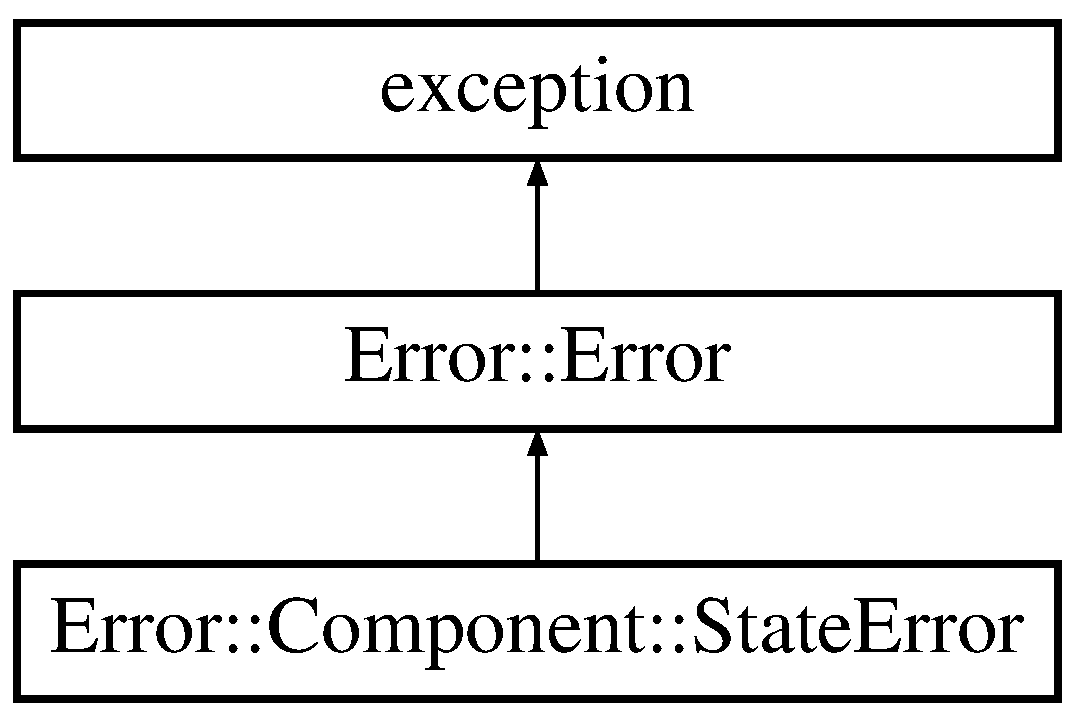
\includegraphics[height=3.000000cm]{classError_1_1Component_1_1StateError}
\end{center}
\end{figure}
\subsection*{Public Member Functions}
\begin{DoxyCompactItemize}
\item 
\mbox{\Hypertarget{classError_1_1Component_1_1StateError_a856431742c76b2631bc17c367b34a0f4}\label{classError_1_1Component_1_1StateError_a856431742c76b2631bc17c367b34a0f4}} 
{\bfseries State\+Error} (std\+::string const \&message, std\+::string const \&where=\char`\"{}Unknown\char`\"{})
\end{DoxyCompactItemize}
\subsection*{Additional Inherited Members}


The documentation for this class was generated from the following file\+:\begin{DoxyCompactItemize}
\item 
Include/Error.\+hpp\end{DoxyCompactItemize}

\hypertarget{classTrue}{}\section{True Class Reference}
\label{classTrue}\index{True@{True}}
Inheritance diagram for True\+:\begin{figure}[H]
\begin{center}
\leavevmode
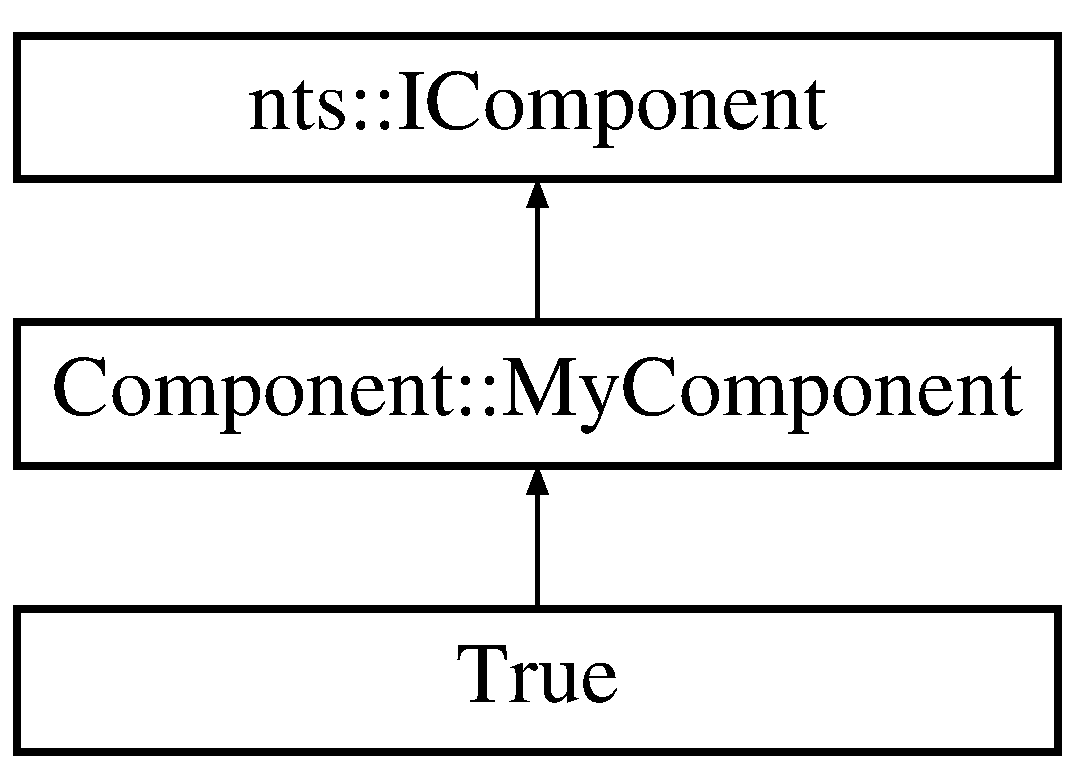
\includegraphics[height=3.000000cm]{classTrue}
\end{center}
\end{figure}
\subsection*{Public Member Functions}
\begin{DoxyCompactItemize}
\item 
\mbox{\Hypertarget{classTrue_a762c7806c6ace768f9a1f7c724ada182}\label{classTrue_a762c7806c6ace768f9a1f7c724ada182}} 
nts\+::\+Tristate {\bfseries compute} (std\+::size\+\_\+t pin=1) override
\item 
\mbox{\Hypertarget{classTrue_af72a9e52f4e3d29eef4c818ebe872c6d}\label{classTrue_af72a9e52f4e3d29eef4c818ebe872c6d}} 
void {\bfseries set\+Link} (std\+::size\+\_\+t pin, \mbox{\hyperlink{classnts_1_1IComponent}{nts\+::\+I\+Component}} \&other, std\+::size\+\_\+t other\+Pin) override
\item 
\mbox{\Hypertarget{classTrue_aed162ed29974c70e20c69e67bfad62c4}\label{classTrue_aed162ed29974c70e20c69e67bfad62c4}} 
void {\bfseries dump} () const noexcept override
\item 
\mbox{\Hypertarget{classTrue_aac91f7cef8337ca9bd9d5ed309e18db7}\label{classTrue_aac91f7cef8337ca9bd9d5ed309e18db7}} 
void {\bfseries set\+Input} (std\+::size\+\_\+t pin, \mbox{\hyperlink{classnts_1_1IComponent}{nts\+::\+I\+Component}} \&other, std\+::size\+\_\+t other\+Pin) final
\item 
\mbox{\Hypertarget{classTrue_aae98876cf193e0a4c4a8d79aad6872a5}\label{classTrue_aae98876cf193e0a4c4a8d79aad6872a5}} 
void {\bfseries set\+Output} (std\+::size\+\_\+t pin, \mbox{\hyperlink{classnts_1_1IComponent}{nts\+::\+I\+Component}} \&other, std\+::size\+\_\+t other\+Pin) final
\end{DoxyCompactItemize}
\subsection*{Additional Inherited Members}


The documentation for this class was generated from the following files\+:\begin{DoxyCompactItemize}
\item 
Include/True.\+hpp\item 
Src/\+Components/True.\+cpp\end{DoxyCompactItemize}

\chapter{File Documentation}
\hypertarget{C4001_8hpp}{}\section{Include/\+C4001.hpp File Reference}
\label{C4001_8hpp}\index{Include/\+C4001.\+hpp@{Include/\+C4001.\+hpp}}


\mbox{\hyperlink{classC4001}{C4001}} class.  


{\ttfamily \#include \char`\"{}I\+Component.\+hpp\char`\"{}}\newline
{\ttfamily \#include \char`\"{}Component.\+hpp\char`\"{}}\newline
{\ttfamily \#include $<$iostream$>$}\newline
{\ttfamily \#include $<$string$>$}\newline
{\ttfamily \#include $<$map$>$}\newline
\subsection*{Classes}
\begin{DoxyCompactItemize}
\item 
class \mbox{\hyperlink{classC4001}{C4001}}
\begin{DoxyCompactList}\small\item\em Quad 2-\/input N\+OR gate. \end{DoxyCompactList}\end{DoxyCompactItemize}


\subsection{Detailed Description}
\mbox{\hyperlink{classC4001}{C4001}} class. 

\begin{DoxyAuthor}{Author}
Cécile C\+A\+D\+O\+UL 

Florent P\+O\+I\+N\+S\+A\+RD 
\end{DoxyAuthor}

\hypertarget{C4011_8hpp}{}\section{Include/\+C4011.hpp File Reference}
\label{C4011_8hpp}\index{Include/\+C4011.\+hpp@{Include/\+C4011.\+hpp}}


\mbox{\hyperlink{classC4011}{C4011}} class.  


{\ttfamily \#include \char`\"{}I\+Component.\+hpp\char`\"{}}\newline
{\ttfamily \#include \char`\"{}Component.\+hpp\char`\"{}}\newline
{\ttfamily \#include $<$iostream$>$}\newline
{\ttfamily \#include $<$string$>$}\newline
{\ttfamily \#include $<$map$>$}\newline
\subsection*{Classes}
\begin{DoxyCompactItemize}
\item 
class \mbox{\hyperlink{classC4011}{C4011}}
\begin{DoxyCompactList}\small\item\em Quad 2-\/input N\+A\+ND gate. \end{DoxyCompactList}\end{DoxyCompactItemize}


\subsection{Detailed Description}
\mbox{\hyperlink{classC4011}{C4011}} class. 

\begin{DoxyAuthor}{Author}
Cécile C\+A\+D\+O\+UL 

Florent P\+O\+I\+N\+S\+A\+RD 
\end{DoxyAuthor}

\hypertarget{C4030_8hpp}{}\section{Include/\+C4030.hpp File Reference}
\label{C4030_8hpp}\index{Include/\+C4030.\+hpp@{Include/\+C4030.\+hpp}}


\mbox{\hyperlink{classC4030}{C4030}} class.  


{\ttfamily \#include \char`\"{}I\+Component.\+hpp\char`\"{}}\newline
{\ttfamily \#include \char`\"{}Component.\+hpp\char`\"{}}\newline
{\ttfamily \#include $<$iostream$>$}\newline
{\ttfamily \#include $<$string$>$}\newline
{\ttfamily \#include $<$map$>$}\newline
\subsection*{Classes}
\begin{DoxyCompactItemize}
\item 
class \mbox{\hyperlink{classC4030}{C4030}}
\begin{DoxyCompactList}\small\item\em Quad 2-\/input E\+X\+C\+L\+U\+S\+I\+V\+E-\/\+OR gate. \end{DoxyCompactList}\end{DoxyCompactItemize}


\subsection{Detailed Description}
\mbox{\hyperlink{classC4030}{C4030}} class. 

\begin{DoxyAuthor}{Author}
Cécile C\+A\+D\+O\+UL 

Florent P\+O\+I\+N\+S\+A\+RD 
\end{DoxyAuthor}

\hypertarget{C4071_8hpp}{}\section{Include/\+C4071.hpp File Reference}
\label{C4071_8hpp}\index{Include/\+C4071.\+hpp@{Include/\+C4071.\+hpp}}


\mbox{\hyperlink{classC4071}{C4071}} class.  


{\ttfamily \#include \char`\"{}I\+Component.\+hpp\char`\"{}}\newline
{\ttfamily \#include \char`\"{}Component.\+hpp\char`\"{}}\newline
{\ttfamily \#include $<$iostream$>$}\newline
{\ttfamily \#include $<$string$>$}\newline
{\ttfamily \#include $<$map$>$}\newline
\subsection*{Classes}
\begin{DoxyCompactItemize}
\item 
class \mbox{\hyperlink{classC4071}{C4071}}
\begin{DoxyCompactList}\small\item\em Quad 2-\/input OR gate. \end{DoxyCompactList}\end{DoxyCompactItemize}


\subsection{Detailed Description}
\mbox{\hyperlink{classC4071}{C4071}} class. 

\begin{DoxyAuthor}{Author}
Cécile C\+A\+D\+O\+UL 

Florent P\+O\+I\+N\+S\+A\+RD 
\end{DoxyAuthor}

\hypertarget{C4081_8hpp}{}\section{Include/\+C4081.hpp File Reference}
\label{C4081_8hpp}\index{Include/\+C4081.\+hpp@{Include/\+C4081.\+hpp}}


\mbox{\hyperlink{classC4081}{C4081}} class.  


{\ttfamily \#include \char`\"{}I\+Component.\+hpp\char`\"{}}\newline
{\ttfamily \#include \char`\"{}Component.\+hpp\char`\"{}}\newline
{\ttfamily \#include $<$iostream$>$}\newline
{\ttfamily \#include $<$string$>$}\newline
{\ttfamily \#include $<$map$>$}\newline
\subsection*{Classes}
\begin{DoxyCompactItemize}
\item 
class \mbox{\hyperlink{classC4081}{C4081}}
\begin{DoxyCompactList}\small\item\em Quad 2-\/input A\+ND gate. \end{DoxyCompactList}\end{DoxyCompactItemize}


\subsection{Detailed Description}
\mbox{\hyperlink{classC4081}{C4081}} class. 

\begin{DoxyAuthor}{Author}
Cécile C\+A\+D\+O\+UL 

Florent P\+O\+I\+N\+S\+A\+RD 
\end{DoxyAuthor}

%--- End generated contents ---

% Index
\backmatter
\newpage
\phantomsection
\clearemptydoublepage
\addcontentsline{toc}{chapter}{Index}
\printindex

\end{document}
